%%
%% This is file `sample-sigconf.tex',
%% generated with the docstrip utility.
%%
%% The original source files were:
%%
%% samples.dtx  (with options: `all,proceedings,bibtex,sigconf')
%% 
%% IMPORTANT NOTICE:
%% 
%% For the copyright see the source file.
%% 
%% Any modified versions of this file must be renamed
%% with new filenames distinct from sample-sigconf.tex.
%% 
%% For distribution of the original source see the terms
%% for copying and modification in the file samples.dtx.
%% 
%% This generated file may be distributed as long as the
%% original source files, as listed above, are part of the
%% same distribution. (The sources need not necessarily be
%% in the same archive or directory.)
%%
%%
%% Commands for TeXCount
%TC:macro \cite [option:text,text]
%TC:macro \citep [option:text,text]
%TC:macro \citet [option:text,text]
%TC:envir table 0 1
%TC:envir table* 0 1
%TC:envir tabular [ignore] word
%TC:envir displaymath 0 word
%TC:envir math 0 word
%TC:envir comment 0 0
%%
%% The first command in your LaTeX source must be the \documentclass
%% command.
%%
%% For submission and review of your manuscript please change the
%% command to \documentclass[manuscript, screen, review]{acmart}.
%%
%% When submitting camera ready or to TAPS, please change the command
%% to \documentclass[sigconf]{acmart} or whichever template is required
%% for your publication.
%%
%%
\documentclass[sigconf]{acmart}
%%
%% \BibTeX command to typeset BibTeX logo in the docs
\AtBeginDocument{%
  \providecommand\BibTeX{{%
    Bib\TeX}}}
\usepackage{multirow}
\usepackage{pgfplots}
\pgfplotsset{compat=1.18}
\definecolor{RoyalBlue}{RGB}{0, 70, 156}
\definecolor{ScholarRed}{RGB}{160, 0, 0}
\definecolor{ScholarGold}{RGB}{212, 160, 0}
\definecolor{ScholarGreen}{RGB}{0, 105, 60}
\definecolor{ScholarPurple}{RGB}{100, 45, 145}
\definecolor{ScholarTeal}{RGB}{0, 120, 120}
\definecolor{ScholarOrange}{RGB}{200, 90, 0}

%% Rights management information.  This information is sent to you
%% when you complete the rights form.  These commands have SAMPLE
%% values in them; it is your responsibility as an author to replace
%% the commands and values with those provided to you when you
%% complete the rights form.
\settopmatter{printacmref=false, authorsperrow=4} % 移除 ACM Reference Format 並強制每排 4 位作者
\setcopyright{none}           % 移除版權宣告與分隔線
\renewcommand\footnotetextcopyrightpermission[1]{} % 強制隱藏底部許可文字


%%
%% Submission ID.
%% Use this when submitting an article to a sponsored event. You'll
%% receive a unique submission ID from the organizers
%% of the event, and this ID should be used as the parameter to this command.
%%\acmSubmissionID{123-A56-BU3}

%%
%% For managing citations, it is recommended to use bibliography
%% files in BibTeX format.
%%
%% You can then either use BibTeX with the ACM-Reference-Format style,
%% or BibLaTeX with the acmnumeric or acmauthoryear sytles, that include
%% support for advanced citation of software artefact from the
%% biblatex-software package, also separately available on CTAN.
%%
%% Look at the sample-*-biblatex.tex files for templates showcasing
%% the biblatex styles.
%%

%%
%% The majority of ACM publications use numbered citations and
%% references.  The command \citestyle{authoryear} switches to the
%% "author year" style.
%%
%% If you are preparing content for an event
%% sponsored by ACM SIGGRAPH, you must use the "author year" style of
%% citations and references.
%% Uncommenting
%% the next command will enable that style.
%%\citestyle{acmauthoryear}


%%
%% end of the preamble, start of the body of the document source.
\begin{document}

%%
%% The "title" command has an optional parameter,
%% allowing the author to define a "short title" to be used in page headers.
\title{Handling Imbalanced Data in Binary Classification: A Review and Comparative Experimental Study}

%%
%% The "author" command and its associated commands are used to define
%% the authors and their affiliations.
%% Of note is the shared affiliation of the first two authors, and the
%% "authornote" and "authornotemark" commands
%% used to denote shared contribution to the research.
%% --- 四位作者並排排版 ---
\author{Chi-Wei, PENG}
\affiliation{\institution{114423004} \country{}}
\email{114423004@cc.ncu.edu.tw}

\author{Ting-Chun, Lin}
\affiliation{\institution{114423009} \country{}}
\email{Tinalin@g.ncu.edu.tw}

\author{Chiu-Hsiang, Lin}
\affiliation{\institution{114423049} \country{}}
\email{114423049@cc.ncu.edu.tw}

\author{Chia-Chen, Lee}
\affiliation{\institution{114423050} \country{}}
\email{cclee@g.ncu.edu.tw}

%%
%% By default, the full list of authors will be used in the page
%% headers. Often, this list is too long, and will overlap
%% other information printed in the page headers. This command allows
%% the author to define a more concise list
%% of authors' names for this purpose.
\renewcommand{\shortauthors}{Trovato et al.}

%%
%% The abstract is a short summary of the work to be presented in the
%% article.
\begin{abstract}
  add later...
\end{abstract}

% CCS Concepts and Keywords
\keywords{Imbalanced Data, Resampling Methods, Boosting Algorithms, Machine Learning}
%% A "teaser" image appears between the author and affiliation
%% information and the body of the document, and typically spans the
%% page.


\received{20 February 2007}
\received[revised]{12 March 2009}
\received[accepted]{5 June 2009}

%%
%% This command processes the author and affiliation and title
%% information and builds the first part of the formatted document.
\maketitle

\section{Introduction}

\subsection{Background and Problem Definition}
In recent years, the rapid expansion of data availability across large-scale, complex, and networked systems has propelled machine learning to prominent roles in numerous application domains [1].

However, real-world data distributions are inherently complex and frequently exhibit a significant class imbalance. The class imbalance problem arises when the number of instances belonging to one class (the majority class) substantially outnumbers those of another (the minority class), resulting in a severely skewed training distribution [1, 2].

This phenomenon is pervasive in many high-stakes domains, including financial fraud detection, network intrusion detection, and the diagnosis of rare diseases such as diabetes and stroke, where the minority class---despite its low frequency of occurrence---typically constitutes the primary target of predictive interest [3, 4].

\subsection{Challenges and the Pitfalls of Evaluation Metrics}
Standard machine learning models are generally designed under the implicit assumption of an approximately balanced class distribution. Consequently, when applied to skewed data, these models exhibit a systematic bias toward the majority class, yielding poor predictive performance for minority instances---precisely those of greatest practical concern [1].

This issue is further compounded by the widespread use of conventional evaluation metrics. Overall accuracy, in particular, is highly misleading under class imbalance: a naive classifier that assigns all instances to the majority class can attain superficially high accuracy while entirely failing to identify any minority-class example [5].

To overcome this limitation, the research community has advocated the adoption of more discriminative metrics, including the F1-Score, the Area Under the Receiver Operating Characteristic Curve (AUC-ROC) [6], and the Geometric Mean (G-Mean) [7], which collectively provide a more faithful assessment of model performance across both classes.

\subsection{Taxonomy of Imbalanced Learning Techniques}
To address the challenges posed by imbalanced datasets, a rich body of literature has proposed numerous techniques, which are broadly categorized into three main families: data-level methods, algorithmic-level methods, and hybrid strategies [1, 8].

Data-level approaches modify the training data distribution prior to model induction, either by oversampling the minority class---most notably through the Synthetic Minority Over-sampling Technique (SMOTE) [2] and its variants---or by undersampling the majority class through methods such as Random Under-Sampling (RUS).

Algorithmic-level approaches, by contrast, leave the data distribution unchanged and instead modify the learning procedure itself; representative techniques include cost-sensitive learning and ensemble-based methods such as weighted classifiers and boosting frameworks [9].

Finally, hybrid strategies combine the complementary strengths of both data resampling and algorithmic robustness, with methods such as SMOTEBoost and RUSBoost serving as prominent examples [9].

\subsection{Research Gap and Objectives}
Despite the substantial volume of existing work, many comparative studies evaluate imbalanced learning techniques across heterogeneous datasets that vary simultaneously in multiple dimensions---including class overlap, feature complexity, and sample size---making it difficult to isolate the independent effect of the Imbalance Ratio (IR) on classifier performance [1]. Confounding factors of this nature limit the interpretability of empirical findings and reduce their practical utility as guidelines for practitioners.

To address this gap, this study proposes a rigorous empirical framework grounded in controlled experimental design. Rather than relying solely on a diverse collection of independent datasets, we systematically vary the IR within a curated set of benchmark datasets spanning a wide range of imbalance severity---from mild (IR $\approx$ 2.4) to extreme (IR $\approx$ 41.4)---thereby enabling direct, controlled comparisons across escalating levels of class imbalance.

Within this framework, we conduct a systematic evaluation of representative methods from all three technique families---data-level, algorithmic-level, and hybrid---using three established base classifiers (SVM, Random Forest, and XGBoost) and a comprehensive set of evaluation metrics (F1-Score, AUC-ROC, and G-Mean). By analyzing the performance degradation trajectories of each strategy as class imbalance worsens, this study aims to provide both a nuanced empirical understanding of the strengths and limitations of existing approaches and actionable practical guidance for selecting appropriate imbalanced learning techniques in binary classification tasks.

\section{Method}
\label{sec:method}

\subsection{Data-level Methods}
At the data pre-processing stage, techniques for addressing class imbalance can be broadly categorized into two types: non-synthetic and synthetic methods. Non-synthetic methods adjust the class distribution using existing data, leaving the underlying information unaltered. Conversely, synthetic methods mitigate the imbalance by generating new data samples using existing features.

\subsubsection{Non-synthetic method}
\paragraph{(i) Random sampling:} Resampling strategies generally include techniques such as under-sampling, over-sampling, and hybrid sampling. Random under-sampling (RUS) deletes samples from the majority class, which may discard useful data. Random over-sampling (ROS) achieves dataset balance by duplicating minority class samples, but this exact duplication increases the risk of overfitting. [81, 10]

In most cases, under-sampling improves model performance more effectively than over-sampling. However, in certain specific scenarios—such as when the negative class is dominant—the opposite holds true. The optimal resampling ratio varies depending on the dataset and the chosen resampling strategy, rather than simply supplementing or reducing classes to a perfectly balanced state. [44, 11]

\paragraph{(ii) Hybrid sampling:} Hybrid sampling combines the advantages of both over-sampling and under-sampling while mitigating their respective disadvantages. Applying over-sampling before under-sampling generally yields better performance than the reverse order. However, the hybrid sampling ratio must be determined manually, often requiring domain knowledge. If this ratio is inappropriately set for a given dataset, the approach may fail to show the benefits of hybridization and could even perform worse than using either technique alone. [12]

\section{EXPERIMENTAL SETUP}

\subsection{Datasets}

To rigorously investigate the effect of varying Imbalance Ratios~(IR) on
classifier performance, this study employs eight benchmark datasets sourced
from the KEEL (Knowledge Extraction based on Evolutionary Learning)
repository~\cite{alcala2011keel}, a widely adopted resource for imbalanced
classification research.
The selected datasets span a broad spectrum of imbalance severity---from
mild to extreme---and originate from diverse real-world domains, thereby
enabling controlled cross-IR comparisons while maintaining ecological
validity.

The Imbalance Ratio is defined formally as:
%
\begin{equation}
  \mathrm{IR} = \frac{|S_{\mathrm{maj}}|}{|S_{\mathrm{min}}|},
  \label{eq:IR}
\end{equation}
%
where $|S_{\mathrm{maj}}|$ and $|S_{\mathrm{min}}|$ denote the cardinalities
of the majority and minority classes, respectively.
Following the severity categorization proposed in the imbalanced learning
literature~\cite{he2009learning}, the datasets are stratified into four
levels: \emph{mild} ($\mathrm{IR} < 3$), \emph{moderate}
($3 \le \mathrm{IR} < 15$), \emph{severe} ($15 \le \mathrm{IR} < 30$),
and \emph{extreme} ($\mathrm{IR} \ge 30$).

All experiments employ \textbf{stratified 5-fold cross-validation} to
ensure that the class distribution is preserved in every fold.
The complete characteristics of the benchmark suite are summarised in
Table~\ref{tab:datasets}.

% ---------- Table 1 ----------
\begin{table*}[t]
  \centering
  \caption{Summary of Benchmark Datasets.}
  \label{tab:datasets}
  \small
  \setlength{\tabcolsep}{12pt} 
  \begin{tabular}{lrrrrrl}
    \toprule
    \textbf{Dataset} & \textbf{Instances} & \textbf{Features} & \textbf{Minority} & \textbf{Majority} & \textbf{Imbalance Ratio} & \textbf{Severity} \\
    \midrule
    Yeast-1 & 1{,}484 & 8 & 429 & 1{,}055 & 2.46 & Mild     \\
    Yeast-3 & 1{,}484 & 8 & 163 & 1{,}321 & 8.10 & Moderate \\
    Yeast-4 & 1{,}484 & 8 &  51 & 1{,}433 & 28.10 & Severe   \\
    Yeast-6 & 1{,}484 & 8 &  35 & 1{,}449 & 41.40 & Extreme  \\
    \bottomrule
  \end{tabular}
\end{table*}
% ---------- End Table 1 ----------

The inclusion of four Yeast variants (Yeast-1, -3, -4, and -6) sharing an
identical feature space and sample size ($n = 1{,}484$) is a deliberate
methodological choice: by holding feature complexity and data size constant
while varying only the IR, these four datasets allow the direct isolation of
class imbalance severity as the sole experimental variable, effectively
controlling for confounds that commonly hinder cross-dataset
comparisons~\cite{he2009learning}.

\subsection{Evaluation Metrics}

A central challenge in evaluating classifiers on imbalanced datasets is
metric selection.
As demonstrated by He and Garcia~\cite{he2009learning} and mathematically
formalised by Luque~et~al.~\cite{luque2019impact}, overall \emph{Accuracy}
is a fundamentally flawed metric under class imbalance: a degenerate
classifier that assigns every instance to the majority class can attain
superficially high accuracy while entirely failing to detect any
minority-class example.
Accordingly, this study excludes Accuracy as a primary performance measure
and instead adopts a suite of imbalance-aware metrics grounded in the binary
confusion matrix, whose elements are defined as follows: True Positives
(TP), True Negatives (TN), False Positives (FP), and False Negatives (FN),
where the \emph{positive} class denotes the minority class throughout.

\paragraph{Precision and Recall.}
Precision measures the proportion of predicted positive instances that are
truly positive; Recall (Sensitivity) measures the proportion of actual
positive instances that are correctly identified.
Both metrics are defined over the minority class and are expressed
as~\cite{sokolova2009systematic}:
%
\begin{equation}
  \mathrm{Precision} = \frac{TP}{TP + FP},
  \label{eq:precision}
\end{equation}
%
\begin{equation}
  \mathrm{Recall} = \frac{TP}{TP + FN}.
  \label{eq:recall}
\end{equation}

\paragraph{F1-Score.}
The F1-Score is the harmonic mean of Precision and Recall, providing a
single scalar that penalises severe imbalances between the
two~\cite{goutte2005probabilistic}:
%
\begin{equation}
  F_1
    = 2 \cdot \frac{\mathrm{Precision} \times \mathrm{Recall}}
                   {\mathrm{Precision} + \mathrm{Recall}}
    = \frac{2\,TP}{2\,TP + FP + FN}.
  \label{eq:f1}
\end{equation}
%
Because the harmonic mean is strictly lower than the arithmetic mean
whenever Precision and Recall diverge, $F_1$ constitutes a conservative and
informative composite measure for imbalanced classification tasks.

\paragraph{AUC-ROC.}
The Area Under the Receiver Operating Characteristic Curve (AUC-ROC) is a
threshold-independent metric that quantifies a classifier's ability to
discriminate between classes across all possible decision
thresholds~\cite{fawcett2006roc}.
Let the False Positive Rate (FPR) and True Positive Rate (TPR) be defined
as:
%
\begin{equation}
  \mathrm{FPR} = \frac{FP}{FP + TN},
  \qquad
  \mathrm{TPR} = \frac{TP}{TP + FN}.
  \label{eq:fpr_tpr}
\end{equation}
%
The AUC-ROC is then computed as:
%
\begin{equation}
  \mathrm{AUC}_{\mathrm{ROC}}
    = \int_{0}^{1} \mathrm{TPR}\!\left(\mathrm{FPR}^{-1}(x)\right) dx.
  \label{eq:aucroc}
\end{equation}
%
A value of $0.5$ corresponds to random classification, while $1.0$ denotes
a perfect classifier.
As noted by Saito and Rehmsmeier~\cite{saito2015precision}, however,
ROC-based metrics can present an overly optimistic picture under extreme
class imbalance, because the large pool of true negatives in the majority
class suppresses the FPR, thereby inflating the apparent curve.

\paragraph{G-Mean.}
The Geometric Mean (G-Mean), originally proposed by Kubat and
Matwin~\cite{kubat1997addressing} for imbalanced learning, is the square
root of the product of Sensitivity (Recall) and Specificity.
It provides a balanced assessment of performance across both classes
simultaneously: poor performance on \emph{either} class leads to a sharp
decline in the overall score.
Specificity and G-Mean are defined as:
%
\begin{equation}
  \mathrm{Specificity} = \frac{TN}{TN + FP},
  \label{eq:specificity}
\end{equation}
%
\begin{equation}
  \mathrm{G\text{-}Mean}
    = \sqrt{\mathrm{Recall} \times \mathrm{Specificity}}
    = \sqrt{\frac{TP}{TP + FN} \cdot \frac{TN}{TN + FP}}.
  \label{eq:gmean}
\end{equation}

\paragraph{Metric Selection Rationale.}
Although this study reports all metrics described above for completeness,
the \textbf{primary evaluation metrics are F1-Score, AUC-ROC, and G-Mean}.
These three are selected because they collectively capture complementary
dimensions of classifier performance under imbalance: the F1-Score reflects
the precision--recall trade-off for the minority class; the AUC-ROC captures
threshold-independent ranking ability across all decision boundaries; and
the G-Mean ensures that majority-class performance is not sacrificed for
minority-class gains.
primary comparisons, in accordance with the limitations identified in prior literature~\cite{he2009learning, luque2019impact, saito2015precision}.

\section{Experimental Results Summary}

This section provides a comprehensive summary of the experimental results across all evaluated methods and datasets.

\section{Detailed Experimental Analysis}
\label{sec:experimental_analysis}

In this section, we provide a detailed analysis of the experimental results, categorized by the level of intervention: data-level, algorithm-level, and hybrid strategies.

\begin{table*}[t]
  \centering
  \caption{Comprehensive Experimental Results Summary across all methodology levels.}
  \label{tab:comprehensive_summary}
  \footnotesize
  \setlength{\tabcolsep}{3.5pt}
  \begin{tabular}{llcccccccccc}
    \toprule
    \textbf{Type} & \textbf{Method} & \textbf{Dataset} & \textbf{Acc.} & \textbf{Prec.} & \textbf{Rec.} & \textbf{F1} & \textbf{AUC} & \textbf{PR-AUC} & \textbf{G-Mean} & \textbf{BAcc.} \\
    \midrule
    \multirow{16}{*}{Data Level} & \multirow{4}{*}{Baseline} 
    & yeast1 & 0.7581 & 0.6410 & 0.4025 & 0.4850 & 0.7881 & 0.5887 & 0.5976 & 0.6526 \\
    & & yeast3 & 0.9477 & 0.8106 & 0.6848 & 0.7412 & 0.9570 & 0.7924 & 0.8184 & 0.8325 \\
    & & yeast4 & 0.9661 & 0.3556 & 0.0970 & 0.1403 & 0.8561 & 0.3739 & 0.2219 & 0.5470 \\
    & & yeast6 & 0.9798 & 0.4556 & 0.2952 & 0.3445 & 0.8999 & 0.5656 & 0.4296 & 0.6458 \\
    \cmidrule{2-11}
    & \multirow{4}{*}{oversampling} 
    & yeast1 & 0.7280 & 0.5356 & 0.6596 & 0.5841 & 0.7835 & 0.5737 & 0.7021 & 0.7077 \\
    & & yeast3 & 0.9292 & 0.6479 & 0.8488 & 0.7290 & 0.9509 & 0.7530 & 0.8920 & 0.8940 \\
    & & yeast4 & 0.9261 & 0.3308 & 0.4897 & 0.3022 & 0.8732 & 0.3626 & 0.6272 & 0.7157 \\
    & & yeast6 & 0.9537 & 0.3796 & 0.6857 & 0.4355 & 0.9080 & 0.4895 & 0.7952 & 0.8230 \\
    \cmidrule{2-11}
    & \multirow{4}{*}{SMOTE} 
    & yeast1 & 0.7201 & 0.5209 & 0.6760 & 0.5831 & 0.7834 & 0.5747 & 0.7029 & 0.7070 \\
    & & yeast3 & 0.9328 & 0.6561 & 0.8551 & 0.7391 & 0.9571 & 0.7664 & 0.8971 & 0.8988 \\
    & & yeast4 & 0.9115 & 0.2465 & 0.6152 & 0.3315 & 0.8801 & 0.3527 & 0.7406 & 0.7686 \\
    & & yeast6 & 0.9452 & 0.3202 & 0.7333 & 0.4155 & 0.9240 & 0.4788 & 0.8248 & 0.8418 \\
    \cmidrule{2-11}
    & \multirow{4}{*}{SMOTE-ENN} 
    & yeast1 & 0.6734 & 0.4657 & 0.7948 & 0.5846 & 0.7803 & 0.5666 & 0.7011 & 0.7094 \\
    & & yeast3 & 0.9216 & 0.6028 & 0.8938 & 0.7177 & 0.9533 & 0.7438 & 0.9089 & 0.9094 \\
    & & yeast4 & 0.8821 & 0.1900 & 0.6921 & 0.2928 & 0.8881 & 0.3371 & 0.7769 & 0.7905 \\
    & & yeast6 & 0.9306 & 0.2587 & 0.7810 & 0.3724 & 0.9324 & 0.4875 & 0.8468 & 0.8576 \\
    \midrule
    \multirow{24}{*}{Algorithm Level} & \multirow{4}{*}{RandomForest} 
    & yeast1 & 0.7783 & 0.6650 & 0.4803 & 0.5553 & 0.8133 & 0.6435 & 0.6561 & 0.6899 \\
    & & yeast3 & 0.9447 & 0.7870 & 0.6805 & 0.7275 & 0.9706 & 0.8316 & 0.8134 & 0.8289 \\
    & & yeast4 & 0.9677 & 0.6000 & 0.1364 & 0.2062 & 0.9206 & 0.4073 & 0.3206 & 0.5668 \\
    & & yeast6 & 0.9831 & 0.7667 & 0.4000 & 0.5054 & 0.8997 & 0.5629 & 0.6088 & 0.6986 \\
    \cmidrule{2-11}
    & \multirow{4}{*}{\begin{tabular}[c]{@{}l@{}}CS-\\RandomForest\end{tabular}} 
    & yeast1 & 0.7891 & 0.6979 & 0.4825 & 0.5688 & 0.8114 & 0.6420 & 0.6632 & 0.6981 \\
    & & yeast3 & 0.9461 & 0.7896 & 0.6992 & 0.7396 & 0.9726 & 0.8479 & 0.8254 & 0.8379 \\
    & & yeast4 & 0.9650 & 0.3333 & 0.1164 & 0.1655 & 0.9269 & 0.4298 & 0.2572 & 0.5557 \\
    & & yeast6 & 0.9838 & 0.8667 & 0.4286 & 0.5305 & 0.8965 & 0.5907 & 0.6350 & 0.7129 \\
    \cmidrule{2-11}
    & \multirow{4}{*}{XGBoost} 
    & yeast1 & 0.7648 & 0.6122 & 0.5151 & 0.5569 & 0.7847 & 0.6034 & 0.6662 & 0.6907 \\
    & & yeast3 & 0.9434 & 0.7567 & 0.7176 & 0.7354 & 0.9612 & 0.7726 & 0.8338 & 0.8444 \\
    & & yeast4 & 0.9629 & 0.4503 & 0.2764 & 0.3241 & 0.9165 & 0.3767 & 0.5024 & 0.6319 \\
    & & yeast6 & 0.9771 & 0.5267 & 0.4857 & 0.4992 & 0.9246 & 0.5340 & 0.6875 & 0.7373 \\
    \cmidrule{2-11}
    & \multirow{4}{*}{\begin{tabular}[c]{@{}l@{}}CS-\\XGBoost\end{tabular}} 
    & yeast1 & 0.7561 & 0.5765 & 0.5989 & 0.5861 & 0.7859 & 0.6012 & 0.6998 & 0.7094 \\
    & & yeast3 & 0.9468 & 0.7482 & 0.7852 & 0.7649 & 0.9615 & 0.7895 & 0.8709 & 0.8760 \\
    & & yeast4 & 0.9582 & 0.4230 & 0.3945 & 0.3932 & 0.9107 & 0.4053 & 0.6066 & 0.6865 \\
    & & yeast6 & 0.9764 & 0.4984 & 0.5714 & 0.5294 & 0.9242 & 0.5515 & 0.7399 & 0.7788 \\
    \cmidrule{2-11}
    & \multirow{4}{*}{AdaBoost (d=1)} 
    & yeast1 & 0.7601 & 0.6293 & 0.4219 & 0.5045 & 0.7878 & 0.5760 & 0.6152 & 0.6598 \\
    & & yeast3 & 0.9508 & 0.7891 & 0.7725 & 0.7770 & 0.9721 & 0.7808 & 0.8664 & 0.8726 \\
    & & yeast4 & 0.9623 & 0.3500 & 0.1945 & 0.2439 & 0.9217 & 0.3758 & 0.3814 & 0.5920 \\
    & & yeast6 & 0.9831 & 0.7000 & 0.4857 & 0.5655 & 0.9380 & 0.5549 & 0.6836 & 0.7404 \\
    \cmidrule{2-11}
    & \multirow{4}{*}{\begin{tabular}[c]{@{}l@{}}CS-\\AdaBoost\end{tabular}} 
    & yeast1 & 0.6658 & 0.4496 & 0.6922 & 0.5449 & 0.6736 & 0.4009 & 0.6729 & 0.6736 \\
    & & yeast3 & 0.8956 & 0.5169 & 0.9203 & 0.6610 & 0.9470 & 0.7058 & 0.9061 & 0.9064 \\
    & & yeast4 & 0.8922 & 0.2093 & 0.7436 & 0.3251 & 0.9190 & 0.2352 & 0.8154 & 0.8205 \\
    & & yeast6 & 0.8956 & 0.1608 & 0.8000 & 0.2655 & 0.8972 & 0.2441 & 0.8374 & 0.8489 \\
    \midrule
    \multirow{24}{*}{Hybrid Method} & \multirow{4}{*}{AdaBoost (d=5)} 
    & yeast1 & 0.7540 & 0.5853 & 0.5196 & 0.5470 & 0.7821 & 0.5880 & 0.6612 & 0.6845 \\
    & & yeast3 & 0.9421 & 0.7577 & 0.6928 & 0.7231 & 0.9591 & 0.7695 & 0.8199 & 0.8328 \\
    & & yeast4 & 0.9650 & 0.5500 & 0.1964 & 0.2727 & 0.9312 & 0.4115 & 0.3923 & 0.5943 \\
    & & yeast6 & 0.9778 & 0.5500 & 0.3714 & 0.4392 & 0.8979 & 0.4859 & 0.6043 & 0.6819 \\
    \cmidrule{2-11}
    & \multirow{4}{*}{SMOTEBoost} 
    & yeast1 & 0.7473 & 0.5560 & 0.6294 & 0.5903 & 0.7718 & 0.5543 & 0.7074 & 0.7123 \\
    & & yeast3 & 0.9468 & 0.7530 & 0.7725 & 0.7611 & 0.9596 & 0.7989 & 0.8641 & 0.8704 \\
    & & yeast4 & 0.9535 & 0.3799 & 0.3946 & 0.3730 & 0.9147 & 0.4122 & 0.6148 & 0.6840 \\
    & & yeast6 & 0.9778 & 0.5101 & 0.6286 & 0.5539 & 0.9147 & 0.5500 & 0.7704 & 0.8074 \\
    \cmidrule{2-11}
    & \multirow{4}{*}{RUSBoost} 
    & yeast1 & 0.7156 & 0.5171 & 0.6085 & 0.5498 & 0.7558 & 0.5147 & 0.6728 & 0.6839 \\
    & & yeast3 & 0.9003 & 0.5325 & 0.9203 & 0.6731 & 0.9348 & 0.5969 & 0.9090 & 0.9090 \\
    & & yeast4 & 0.8255 & 0.1469 & 0.8418 & 0.2499 & 0.8847 & 0.1846 & 0.8321 & 0.8333 \\
    & & yeast6 & 0.7864 & 0.0856 & 0.8286 & 0.1548 & 0.8265 & 0.0983 & 0.8009 & 0.8070 \\
    \cmidrule{2-11}
    & \multirow{4}{*}{RHSBoost} 
    & yeast1 & 0.7507 & 0.5613 & 0.6456 & 0.5993 & 0.7910 & 0.5896 & 0.7148 & 0.7195 \\
    & & yeast3 & 0.9191 & 0.5901 & 0.9015 & 0.7115 & 0.9546 & 0.6852 & 0.9111 & 0.9114 \\
    & & yeast4 & 0.8396 & 0.1545 & 0.8036 & 0.2584 & 0.8824 & 0.1807 & 0.8210 & 0.8223 \\
    & & yeast6 & 0.8679 & 0.1359 & 0.8571 & 0.2340 & 0.8675 & 0.1328 & 0.8580 & 0.8627 \\
    \cmidrule{2-11}
    & \multirow{4}{*}{SUBoost} 
    & yeast1 & 0.7224 & 0.5297 & 0.5408 & 0.5277 & 0.7571 & 0.5586 & 0.6512 & 0.6685 \\
    & & yeast3 & 0.9394 & 0.7743 & 0.6267 & 0.6877 & 0.9548 & 0.7286 & 0.7778 & 0.8024 \\
    & & yeast4 & 0.9589 & 0.4417 & 0.2746 & 0.3146 & 0.8879 & 0.3961 & 0.4581 & 0.6289 \\
    & & yeast6 & 0.9771 & 0.5343 & 0.4286 & 0.4462 & 0.8706 & 0.4566 & 0.6227 & 0.7095 \\
    \cmidrule{2-11}
    & \multirow{4}{*}{SMOTECSL} 
    & yeast1 & 0.5492 & 0.3855 & 0.9416 & 0.5470 & 0.7931 & 0.5956 & 0.6053 & 0.6656 \\
    & & yeast3 & 0.8538 & 0.4260 & 0.9510 & 0.5883 & 0.9688 & 0.8093 & 0.8947 & 0.8964 \\
    & & yeast4 & 0.6874 & 0.0877 & 0.8618 & 0.1591 & 0.8535 & 0.1488 & 0.7648 & 0.7715 \\
    & & yeast6 & 0.7540 & 0.0865 & 0.9429 & 0.1573 & 0.9100 & 0.3574 & 0.8363 & 0.8462 \\
    \bottomrule
  \end{tabular}
\end{table*}

\subsection{Data Level Methods}
Data-level methods focus on reslicing the training set to achieve a more balanced distribution. This section presenting the G-Mean performance for individual classifiers and visual analysis of the results.

\begin{table*}[t]
  \centering
  \caption{[Data Level] Summary of Experimental Results (Data-Level Methods)}
  \label{tab:datalevel_summary}
  \scriptsize
  \setlength{\tabcolsep}{3.5pt}
  \begin{tabular}{llccccccccc}
    \toprule
    \textbf{Method} & \textbf{Dataset} & \textbf{Model} & \textbf{Acc.} & \textbf{Prec.} & \textbf{Rec.} & \textbf{F1} & \textbf{AUC} & \textbf{PR-AUC} & \textbf{G-Mean} & \textbf{BAcc} \\
    \midrule
    \multirow{12}{*}{Original} & \multirow{3}{*}{yeast1} & KNN & 0.7392 & 0.5623 & 0.4360 & 0.4904 & 0.7550 & 0.5083 & 0.6120 & 0.6492 \\
    & & RF & 0.7783 & 0.6650 & 0.4800 & 0.5553 & 0.8133 & 0.6435 & 0.6561 & 0.6899 \\
    & & SVM & 0.7568 & 0.6956 & 0.2910 & 0.4092 & 0.7961 & 0.6142 & 0.5246 & 0.6187 \\
    \cmidrule{2-11}
    & \multirow{3}{*}{yeast3} & KNN & 0.9468 & 0.8119 & 0.6750 & 0.7362 & 0.9249 & 0.7188 & 0.8133 & 0.8277 \\
    & & RF & 0.9447 & 0.7870 & 0.6800 & 0.7275 & 0.9706 & 0.8316 & 0.8134 & 0.8289 \\
    & & SVM & 0.9515 & 0.8330 & 0.6990 & 0.7598 & 0.9755 & 0.8268 & 0.8285 & 0.8408 \\
    \cmidrule{2-11}
    & \multirow{3}{*}{yeast4} & KNN & 0.9650 & 0.4667 & 0.1550 & 0.2147 & 0.7944 & 0.2928 & 0.3451 & 0.5741 \\
    & & RF & 0.9677 & 0.6000 & 0.1360 & 0.2062 & 0.9206 & 0.4073 & 0.3206 & 0.5668 \\
    & & SVM & 0.9656 & 0.0000 & 0.0000 & 0.0000 & 0.8532 & 0.4215 & 0.0000 & 0.5000 \\
    \cmidrule{2-11}
    & \multirow{3}{*}{yeast6} & KNN & 0.9798 & 0.6000 & 0.4860 & 0.5281 & 0.8997 & 0.5167 & 0.6801 & 0.7387 \\
    & & RF & 0.9831 & 0.7667 & 0.4000 & 0.5054 & 0.8997 & 0.5629 & 0.6088 & 0.6986 \\
    & & SVM & 0.9764 & 0.0000 & 0.0000 & 0.0000 & 0.9003 & 0.6173 & 0.0000 & 0.5000 \\
    \midrule
    \multirow{12}{*}{Oversampling} & \multirow{3}{*}{yeast1} & KNN & 0.6894 & 0.4727 & 0.6573 & 0.5498 & 0.7382 & 0.4774 & 0.6791 & 0.6799 \\
    & & RF & 0.7763 & 0.6244 & 0.5734 & 0.5964 & 0.8120 & 0.6383 & 0.7007 & 0.7161 \\
    & & SVM & 0.7183 & 0.5098 & 0.7481 & 0.6061 & 0.8003 & 0.6054 & 0.7266 & 0.7271 \\
    \cmidrule{2-11}
    & \multirow{3}{*}{yeast3} & KNN & 0.9131 & 0.5730 & 0.8525 & 0.6838 & 0.9151 & 0.6105 & 0.8855 & 0.8865 \\
    & & RF & 0.9488 & 0.7556 & 0.7917 & 0.7729 & 0.9666 & 0.8332 & 0.8752 & 0.8799 \\
    & & SVM & 0.9259 & 0.6151 & 0.9023 & 0.7303 & 0.9709 & 0.8153 & 0.9153 & 0.9156 \\
    \cmidrule{2-11}
    & \multirow{3}{*}{yeast4} & KNN & 0.9360 & 0.2700 & 0.5491 & 0.3585 & 0.7934 & 0.2407 & 0.7068 & 0.7494 \\
    & & RF & 0.9663 & 0.5444 & 0.1964 & 0.2624 & 0.9276 & 0.4124 & 0.3781 & 0.5950 \\
    & & SVM & 0.8760 & 0.1779 & 0.7236 & 0.2856 & 0.8987 & 0.4346 & 0.7965 & 0.8025 \\
    \cmidrule{2-11}
    & \multirow{3}{*}{yeast6} & KNN & 0.9589 & 0.3262 & 0.7143 & 0.4477 & 0.8954 & 0.3599 & 0.8233 & 0.8395 \\
    & & RF & 0.9805 & 0.5993 & 0.4857 & 0.5177 & 0.8890 & 0.5812 & 0.6752 & 0.7391 \\
    & & SVM & 0.9218 & 0.2134 & 0.8571 & 0.3411 & 0.9397 & 0.5274 & 0.8870 & 0.8903 \\
    \midrule
    \multirow{12}{*}{SMOTE} & \multirow{3}{*}{yeast1} & KNN & 0.6934 & 0.4783 & 0.6691 & 0.5575 & 0.7447 & 0.4872 & 0.6855 & 0.6862 \\
    & & RF & 0.7642 & 0.5911 & 0.6013 & 0.5952 & 0.8043 & 0.6297 & 0.7059 & 0.7158 \\
    & & SVM & 0.7028 & 0.4932 & 0.7575 & 0.5965 & 0.8011 & 0.6070 & 0.7173 & 0.7190 \\
    \cmidrule{2-11}
    & \multirow{3}{*}{yeast3} & KNN & 0.9164 & 0.5817 & 0.8648 & 0.6944 & 0.9330 & 0.6695 & 0.8929 & 0.8938 \\
    & & RF & 0.9481 & 0.7363 & 0.8223 & 0.7766 & 0.9666 & 0.8186 & 0.8898 & 0.8930 \\
    & & SVM & 0.9340 & 0.6502 & 0.8780 & 0.7463 & 0.9715 & 0.8111 & 0.9086 & 0.9095 \\
    \cmidrule{2-11}
    & \multirow{3}{*}{yeast4} & KNN & 0.9036 & 0.2039 & 0.6473 & 0.3077 & 0.8303 & 0.2104 & 0.7571 & 0.7800 \\
    & & RF & 0.9522 & 0.3516 & 0.4745 & 0.3938 & 0.9107 & 0.3857 & 0.6667 & 0.7219 \\
    & & SVM & 0.8787 & 0.1839 & 0.7236 & 0.2929 & 0.8993 & 0.4619 & 0.7980 & 0.8039 \\
    \cmidrule{2-11}
    & \multirow{3}{*}{yeast6} & KNN & 0.9265 & 0.2144 & 0.7714 & 0.3344 & 0.9093 & 0.3032 & 0.8434 & 0.8509 \\
    & & RF & 0.9778 & 0.5167 & 0.6286 & 0.5573 & 0.9183 & 0.5391 & 0.7705 & 0.8074 \\
    & & SVM & 0.9313 & 0.2293 & 0.8000 & 0.3549 & 0.9444 & 0.5942 & 0.8606 & 0.8672 \\
    \midrule
    \multirow{12}{*}{SMOTE+ENN} & \multirow{3}{*}{yeast1} & KNN & 0.6671 & 0.4570 & 0.8042 & 0.5828 & 0.7481 & 0.4748 & 0.7011 & 0.7078 \\
    & & RF & 0.7109 & 0.5007 & 0.7224 & 0.5903 & 0.7973 & 0.6146 & 0.7130 & 0.7143 \\
    & & SVM & 0.6422 & 0.4392 & 0.8577 & 0.5807 & 0.7954 & 0.6105 & 0.6891 & 0.7061 \\
    \cmidrule{2-11}
    & \multirow{3}{*}{yeast3} & KNN & 0.9003 & 0.5288 & 0.8771 & 0.6590 & 0.9222 & 0.6136 & 0.8897 & 0.8901 \\
    & & RF & 0.9394 & 0.6726 & 0.8837 & 0.7628 & 0.9666 & 0.8096 & 0.9141 & 0.9150 \\
    & & SVM & 0.9252 & 0.6070 & 0.9206 & 0.7312 & 0.9712 & 0.8083 & 0.9231 & 0.9232 \\
    \cmidrule{2-11}
    & \multirow{3}{*}{yeast4} & KNN & 0.8760 & 0.1826 & 0.7455 & 0.2929 & 0.8424 & 0.1908 & 0.8071 & 0.8131 \\
    & & RF & 0.9205 & 0.2305 & 0.5691 & 0.3253 & 0.9268 & 0.3933 & 0.7208 & 0.7511 \\
    & & SVM & 0.8497 & 0.1570 & 0.7618 & 0.2600 & 0.8951 & 0.4273 & 0.8029 & 0.8073 \\
    \cmidrule{2-11}
    & \multirow{3}{*}{yeast6} & KNN & 0.9036 & 0.1788 & 0.8286 & 0.2925 & 0.9077 & 0.2530 & 0.8624 & 0.8670 \\
    & & RF & 0.9676 & 0.3899 & 0.6857 & 0.4941 & 0.9457 & 0.5976 & 0.8056 & 0.8301 \\
    & & SVM & 0.9205 & 0.2073 & 0.8286 & 0.3305 & 0.9439 & 0.6119 & 0.8724 & 0.8756 \\
    \bottomrule
  \end{tabular}
\end{table*}

\subsubsection{Experimental Tables: Data-Level Results}
\begin{table}[h]
  \centering
  \caption{[Data Level] G-Mean Performance Comparison for KNN Classifier}
  \label{tab:knn_gmean}
  \small
  \begin{tabular}{lcccc}
    \toprule
    Method & Yeast1 & Yeast3 & Yeast4 & Yeast6 \\
    \midrule
    Original & 0.6120 & 0.8133 & 0.3451 & 0.6801 \\
    Oversampling & 0.6791 & 0.8855 & 0.7068 & 0.8233 \\
    SMOTE & 0.6855 & 0.8929 & 0.7571 & 0.8434 \\
    SMOTE+ENN & 0.7011 & 0.8897 & 0.8071 & 0.8624 \\
    \bottomrule
  \end{tabular}
\end{table}

\begin{table}[h]
  \centering
  \caption{[Data Level] G-Mean Performance Comparison for Random Forest Classifier}
  \label{tab:rf_gmean}
  \small
  \begin{tabular}{lcccc}
    \toprule
    Method & Yeast1 & Yeast3 & Yeast4 & Yeast6 \\
    \midrule
    Original & 0.6561 & 0.8134 & 0.3206 & 0.6088 \\
    Oversampling & 0.7007 & 0.8752 & 0.3781 & 0.6752 \\
    SMOTE & 0.7059 & 0.8898 & 0.6667 & 0.7705 \\
    SMOTE+ENN & 0.7130 & 0.9141 & 0.7208 & 0.8056 \\
    \bottomrule
  \end{tabular}
\end{table}

\begin{table}[h]
  \centering
  \caption{[Data Level] G-Mean Performance Comparison for SVM Classifier}
  \label{tab:svm_gmean}
  \small
  \begin{tabular}{lcccc}
    \toprule
    Method & Yeast1 & Yeast3 & Yeast4 & Yeast6 \\
    \midrule
    Original & 0.5246 & 0.8285 & 0.0000 & 0.0000 \\
    Oversampling & 0.7266 & 0.9153 & 0.7965 & 0.8870 \\
    SMOTE & 0.7173 & 0.9086 & 0.7980 & 0.8606 \\
    SMOTE+ENN & 0.6891 & 0.9231 & 0.8029 & 0.8724 \\
    \bottomrule
  \end{tabular}
\end{table}

\subsubsection{Visual Analysis of Data-Level Methods}
This subcategory compares the G-mean performance across multiple classifiers (KNN, Random Forest, SVM) using different data-resampling techniques. Figures~\ref{fig:yeast1_gmean} through \ref{fig:yeast6_gmean} illustrate the impact of oversampling, SMOTE, and SMOTE+ENN.

\begin{figure}[h]
  \centering
  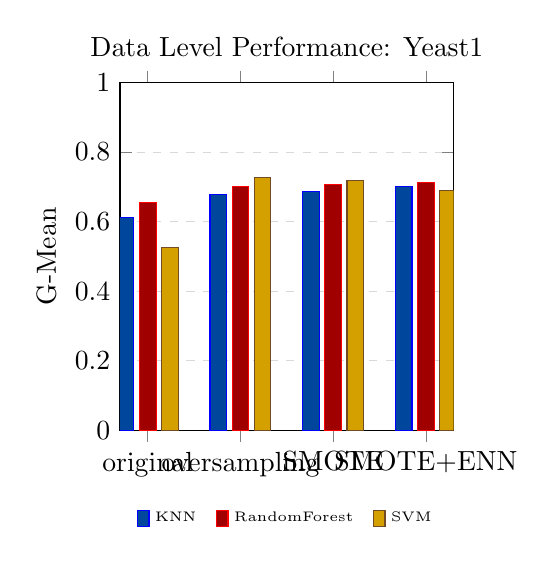
\begin{tikzpicture}
    \begin{axis}[
        ybar,
        height=6cm,
        width=0.48\textwidth,
        bar width=6pt,
        ylabel={G-Mean},
        symbolic x coords={original,oversampling,SMOTE,SMOTE+ENN},
        xtick=data,
        ymin=0, ymax=1.0,
        legend style={at={(0.5,-0.2)}, anchor=north, legend columns=-1, font=\tiny, draw=none, /tikz/every even column/.append style={column sep=5pt}},
        legend image code/.code={\draw[#1] (0cm,-0.1cm) rectangle (0.15cm,0.1cm);},
        ymajorgrids=true,
        grid style={dashed,gray!30},
        title={Data Level Performance: Yeast1},
      ]
      \addplot+ [fill=RoyalBlue] coordinates {(original,0.6120) (oversampling,0.6791) (SMOTE,0.6855) (SMOTE+ENN,0.7011)};
      \addplot+ [fill=ScholarRed] coordinates {(original,0.6561) (oversampling,0.7007) (SMOTE,0.7059) (SMOTE+ENN,0.7130)};
      \addplot+ [fill=ScholarGold] coordinates {(original,0.5246) (oversampling,0.7266) (SMOTE,0.7173) (SMOTE+ENN,0.6891)};
      \legend{KNN, RandomForest, SVM}
    \end{axis}
  \end{tikzpicture}
  \caption{[Data Level] G-Mean performance comparison on Yeast1 dataset.}
  \label{fig:yeast1_gmean}
\end{figure}

\begin{figure}[h]
  \centering
  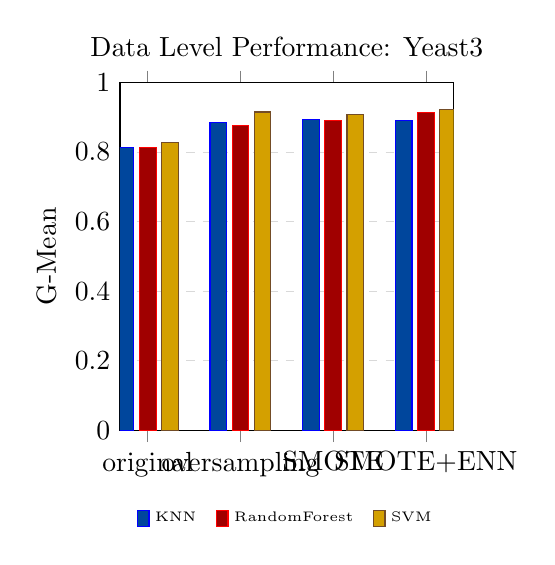
\begin{tikzpicture}
    \begin{axis}[
        ybar,
        height=6cm,
        width=0.48\textwidth,
        bar width=6pt,
        ylabel={G-Mean},
        symbolic x coords={original,oversampling,SMOTE,SMOTE+ENN},
        xtick=data,
        ymin=0, ymax=1.0,
        legend style={at={(0.5,-0.2)}, anchor=north, legend columns=-1, font=\tiny, draw=none, /tikz/every even column/.append style={column sep=5pt}},
        legend image code/.code={\draw[#1] (0cm,-0.1cm) rectangle (0.15cm,0.1cm);},
        ymajorgrids=true,
        grid style={dashed,gray!30},
        title={Data Level Performance: Yeast3},
      ]
      \addplot+ [fill=RoyalBlue] coordinates {(original,0.8133) (oversampling,0.8855) (SMOTE,0.8929) (SMOTE+ENN,0.8897)};
      \addplot+ [fill=ScholarRed] coordinates {(original,0.8134) (oversampling,0.8752) (SMOTE,0.8898) (SMOTE+ENN,0.9141)};
      \addplot+ [fill=ScholarGold] coordinates {(original,0.8285) (oversampling,0.9153) (SMOTE,0.9086) (SMOTE+ENN,0.9231)};
      \legend{KNN, RandomForest, SVM}
    \end{axis}
  \end{tikzpicture}
  \caption{[Data Level] G-Mean performance comparison on Yeast3 dataset.}
  \label{fig:yeast3_gmean}
\end{figure}

\begin{figure}[h]
  \centering
  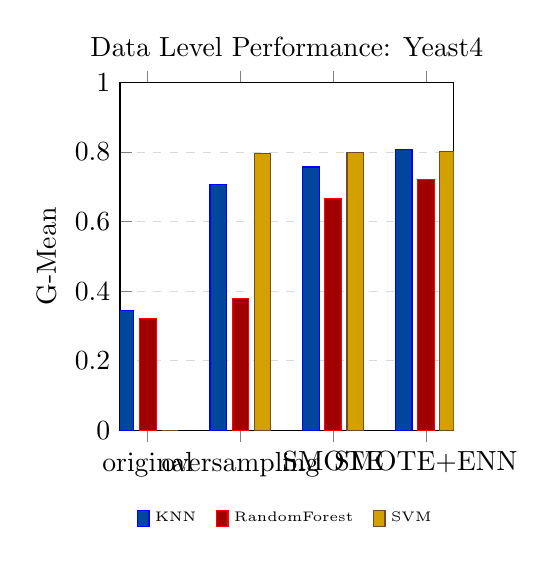
\begin{tikzpicture}
    \begin{axis}[
        ybar,
        height=6cm,
        width=0.48\textwidth,
        bar width=6pt,
        ylabel={G-Mean},
        symbolic x coords={original,oversampling,SMOTE,SMOTE+ENN},
        xtick=data,
        ymin=0, ymax=1.0,
        legend style={at={(0.5,-0.2)}, anchor=north, legend columns=-1, font=\tiny, draw=none, /tikz/every even column/.append style={column sep=5pt}},
        legend image code/.code={\draw[#1] (0cm,-0.1cm) rectangle (0.15cm,0.1cm);},
        ymajorgrids=true,
        grid style={dashed,gray!30},
        title={Data Level Performance: Yeast4},
      ]
      \addplot+ [fill=RoyalBlue] coordinates {(original,0.3451) (oversampling,0.7068) (SMOTE,0.7571) (SMOTE+ENN,0.8071)};
      \addplot+ [fill=ScholarRed] coordinates {(original,0.3206) (oversampling,0.3781) (SMOTE,0.6667) (SMOTE+ENN,0.7208)};
      \addplot+ [fill=ScholarGold] coordinates {(original,0.0000) (oversampling,0.7965) (SMOTE,0.7980) (SMOTE+ENN,0.8029)};
      \legend{KNN, RandomForest, SVM}
    \end{axis}
  \end{tikzpicture}
  \caption{[Data Level] G-Mean performance comparison on Yeast4 dataset.}
  \label{fig:yeast4_gmean}
\end{figure}

\begin{figure}[h]
  \centering
  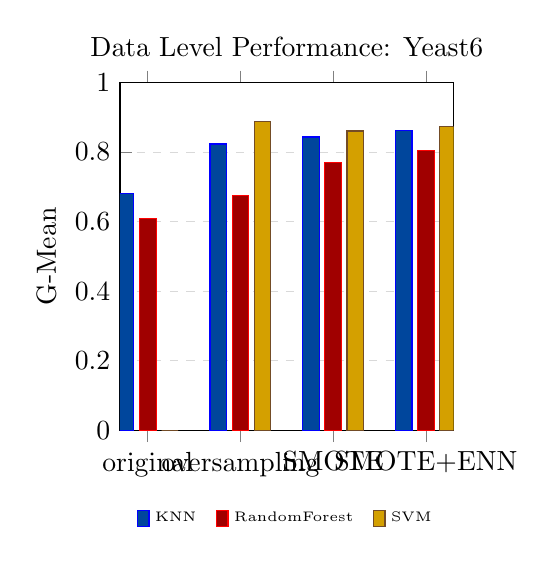
\begin{tikzpicture}
    \begin{axis}[
        ybar,
        height=6cm,
        width=0.48\textwidth,
        bar width=6pt,
        ylabel={G-Mean},
        symbolic x coords={original,oversampling,SMOTE,SMOTE+ENN},
        xtick=data,
        ymin=0, ymax=1.0,
        legend style={at={(0.5,-0.2)}, anchor=north, legend columns=-1, font=\tiny, draw=none, /tikz/every even column/.append style={column sep=5pt}},
        legend image code/.code={\draw[#1] (0cm,-0.1cm) rectangle (0.15cm,0.1cm);},
        ymajorgrids=true,
        grid style={dashed,gray!30},
        title={Data Level Performance: Yeast6},
      ]
      \addplot+ [fill=RoyalBlue] coordinates {(original,0.6801) (oversampling,0.8233) (SMOTE,0.8434) (SMOTE+ENN,0.8624)};
      \addplot+ [fill=ScholarRed] coordinates {(original,0.6088) (oversampling,0.6752) (SMOTE,0.7705) (SMOTE+ENN,0.8056)};
      \addplot+ [fill=ScholarGold] coordinates {(original,0.0000) (oversampling,0.8870) (SMOTE,0.8606) (SMOTE+ENN,0.8724)};
      \legend{KNN, RandomForest, SVM}
    \end{axis}
  \end{tikzpicture}
  \caption{[Data Level] G-Mean performance comparison on Yeast6 dataset.}
  \label{fig:yeast6_gmean}
\end{figure}

\subsection{Algorithm Level Methods}
Algorithm-level methods, such as Cost-Sensitive learning combined with ensemble classifiers (Random Forest, XGBoost, AdaBoost), show higher robustness across varying imbalance ratios by directly internalizing the cost of misclassifying minority instances.

\subsubsection{Visual Analysis of Algorithm-Level Methods}
In this subcategory, we examine the performance shifts in ensemble methods when cost-sensitive mechanisms are applied.

Figure~\ref{fig:algorithm_recall} presents a comparison of Recall scores between standard Random Forest and Weighted (Cost-Sensitive) Random Forest across the Yeast datasets.

\begin{figure}[h]
  \centering
  \Description{Grouped bar chart showing Recall of Random Forest and Weighted Random Forest across four datasets (yeast1, yeast3, yeast4, yeast6).}
  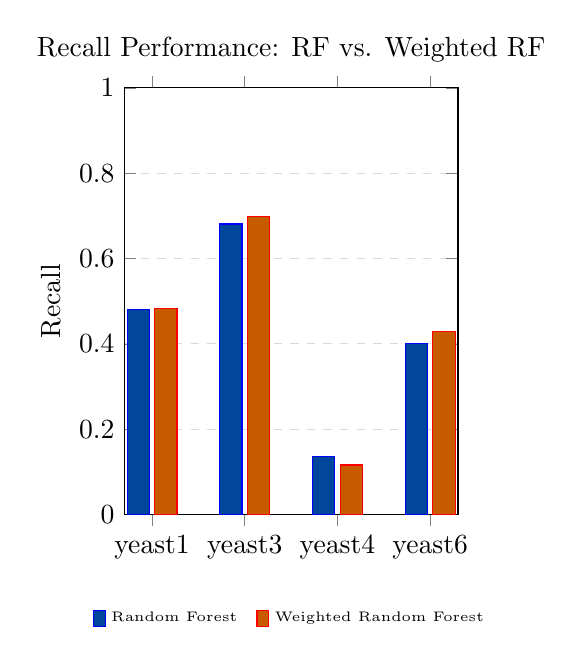
\begin{tikzpicture}
    \begin{axis}[
        ybar,
        height=7cm,
        width=0.48\textwidth,
        bar width=8pt,
        ylabel={Recall},
        symbolic x coords={yeast1,yeast3,yeast4,yeast6},
        xtick=data,
        ymin=0, ymax=1.0,
        legend style={at={(0.5,-0.2)}, anchor=north, legend columns=-1, font=\tiny, draw=none, /tikz/every even column/.append style={column sep=5pt}},
        legend image code/.code={\draw[#1] (0cm,-0.1cm) rectangle (0.15cm,0.1cm);},
        ymajorgrids=true,
        grid style={dashed,gray!30},
        title={Recall Performance: RF vs. Weighted RF},
      ]
      \addplot+ [fill=RoyalBlue] coordinates {(yeast1,0.480) (yeast3,0.681) (yeast4,0.136) (yeast6,0.400)};
      \addplot+ [fill=ScholarOrange] coordinates {(yeast1,0.483) (yeast3,0.699) (yeast4,0.116) (yeast6,0.429)};
      \legend{Random Forest, Weighted Random Forest}
    \end{axis}
  \end{tikzpicture}
  \caption{[Algorithm Level] Recall comparison of standard and weighted Random Forest.}
  \label{fig:algorithm_recall}
\end{figure}

Furthermore, Table~\ref{tab:comprehensive_summary} and Figure~\ref{fig:adaboost_tradeoff} highlight the "death cross" effect in AdaBoost. After applying cost-sensitive weights, Recall improves significantly, but at a severe cost to Precision.

\begin{figure}[h]
    \centering
    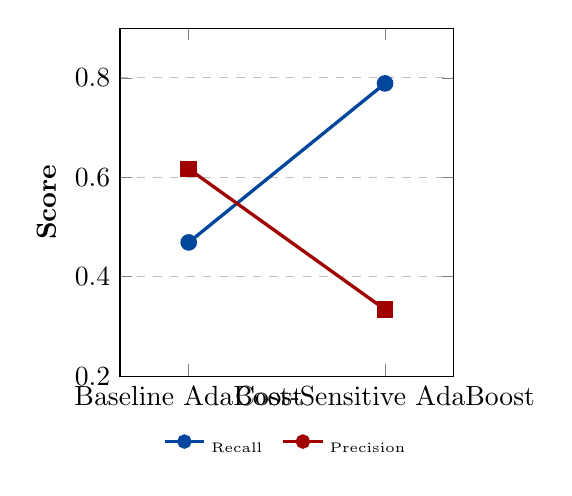
\begin{tikzpicture}
        \begin{axis}[
            width=0.48\textwidth,
            height=6cm,
            ymin=0.2, ymax=0.9,
            ytick={0.2, 0.4, 0.6, 0.8},
            ylabel={\textbf{Score}},
            symbolic x coords={Baseline AdaBoost, Cost-Sensitive AdaBoost},
            xtick=data,
            enlarge x limits=0.35,
            ymajorgrids=true,
            grid style=dashed,
            legend style={at={(0.5,-0.15)}, anchor=north, legend columns=2, font=\tiny, draw=none, /tikz/every even column/.append style={column sep=5pt}},
            legend image code/.code={\draw[#1] (0cm,0.1cm) -- (0.5cm,0.1cm); \fill[#1] (0.25cm,0.1cm) circle (2pt);},
        ]
        \addplot[color=RoyalBlue, mark=*, mark options={scale=1.2}, very thick] coordinates {
            (Baseline AdaBoost, 0.469)
            (Cost-Sensitive AdaBoost, 0.789)
        };
        \addlegendentry{Recall}
        \addplot[color=ScholarRed, mark=square*, mark options={scale=1.2}, very thick] coordinates {
            (Baseline AdaBoost, 0.617)
            (Cost-Sensitive AdaBoost, 0.334)
        };
        \addlegendentry{Precision}
        \end{axis}
    \end{tikzpicture}
    \caption{[Algorithm Level] Dual-metric line chart illustrating the trade-off in AdaBoost.}
    \label{fig:adaboost_tradeoff}
\end{figure}

Finally, the radar chart in Figure~\ref{fig:xgboost_radar} illustrates the balanced improvement across multiple metrics (Recall, Precision, F1-Score, and G-Mean) for XGBoost when cost-sensitive learning is integrated.

\begin{figure}[h]
    \centering
    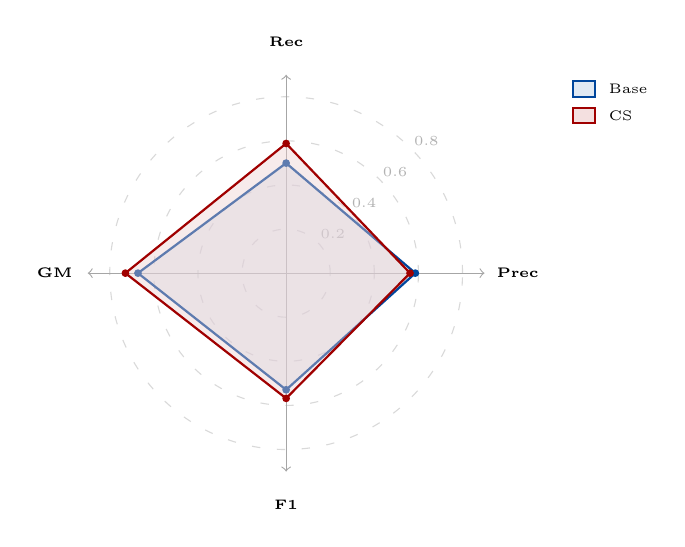
\begin{tikzpicture}[scale=2.8]
        \foreach \r in {0.2, 0.4, 0.6, 0.8} {
            \draw[gray!30, loosely dashed] (0,0) circle (\r);
            \node[gray!60, anchor=south west, inner sep=1pt, font=\tiny] at (45:\r) {\r};
        }
        \foreach \angle/\label in {90/Rec, 0/Prec, 270/F1, 180/GM} {
            \draw[gray!70, ->] (0,0) -- (\angle:0.9);
            \node[font=\tiny\bfseries] at (\angle:1.05) {\label};
        }
        \coordinate (B_Recall)    at (90:0.499);
        \coordinate (B_Precision) at (0:0.586);
        \coordinate (B_F1)        at (270:0.529);
        \coordinate (B_GMean)     at (180:0.672);
        \coordinate (C_Recall)    at (90:0.588);
        \coordinate (C_Precision) at (0:0.562);
        \coordinate (C_F1)        at (270:0.568);
        \coordinate (C_GMean)     at (180:0.729);
        \draw[thick, RoyalBlue, fill=RoyalBlue!20, fill opacity=0.4] (B_Recall) -- (B_Precision) -- (B_F1) -- (B_GMean) -- cycle;
        \foreach \p in {B_Recall, B_Precision, B_F1, B_GMean} { \fill[RoyalBlue] (\p) circle (0.5pt); }
        \draw[thick, ScholarRed, fill=ScholarRed!20, fill opacity=0.4] (C_Recall) -- (C_Precision) -- (C_F1) -- (C_GMean) -- cycle;
        \foreach \p in {C_Recall, C_Precision, C_F1, C_GMean} { \fill[ScholarRed] (\p) circle (0.5pt); }
        \begin{scope}[xshift=1.3cm, yshift=0.8cm]
            \draw[thick, RoyalBlue, fill=RoyalBlue!20, fill opacity=0.6] (0,0) rectangle (0.1, 0.07);
            \node[right, font=\tiny] at (0.12, 0.035) {Base};
            \draw[thick, ScholarRed, fill=ScholarRed!20, fill opacity=0.6] (0,-0.12) rectangle (0.1, -0.05);
            \node[right, font=\tiny] at (0.12, -0.085) {CS};
        \end{scope}
    \end{tikzpicture}
    \caption{[Algorithm Level] Radar Chart comparing Average XGBoost vs. CS-XGBoost.}
    \label{fig:xgboost_radar}
\end{figure}

\subsection{Hybrid Methods}
Hybrid methods integrate data resampling with algorithmic enhancements. This subsection evaluates the efficacy of boosting-based hybrid approaches.

\begin{table}[h]
  \centering
  \caption{[Hybrid Method] Summary of Experimental Results (Boosting-based Methods)}
  \label{tab:hybrid_summary}
  \small
  \begin{tabular}{llccc}
    \toprule
    \textbf{Method} & \textbf{Dataset} & \textbf{F1-score} & \textbf{ROC-AUC} & \textbf{G-Mean} \\
    \midrule
    \multirow{4}{*}{AdaBoost(d=5)} & yeast1 & 0.5470 & 0.7821 & 0.6612 \\
    & yeast3 & 0.7230 & 0.9591 & 0.8199 \\
    & yeast4 & 0.2727 & 0.9312 & 0.3923 \\
    & yeast6 & 0.4392 & 0.8979 & 0.6043 \\
    \cmidrule{1-5}
    \multirow{4}{*}{RHSBoost} & yeast1 & 0.5993 & 0.7910 & 0.7148 \\
    & yeast3 & 0.7115 & 0.9546 & 0.9111 \\
    & yeast4 & 0.2584 & 0.8824 & 0.8210 \\
    & yeast6 & 0.2340 & 0.8675 & 0.8580 \\
    \cmidrule{1-5}
    \multirow{4}{*}{RUSBoost} & yeast1 & 0.5498 & 0.7558 & 0.6728 \\
    & yeast3 & 0.6731 & 0.9348 & 0.9090 \\
    & yeast4 & 0.2499 & 0.8847 & 0.8321 \\
    & yeast6 & 0.1548 & 0.8265 & 0.8009 \\
    \cmidrule{1-5}
    \multirow{4}{*}{SMOTE} & yeast1 & 0.5831 & 0.7834 & 0.7029 \\
    & yeast3 & 0.7391 & 0.9571 & 0.8971 \\
    & yeast4 & 0.3315 & 0.8801 & 0.7406 \\
    & yeast6 & 0.4155 & 0.9240 & 0.8248 \\
    \cmidrule{1-5}
    \multirow{4}{*}{SMOTEBoost} & yeast1 & 0.5903 & 0.7718 & 0.7074 \\
    & yeast3 & 0.7611 & 0.9596 & 0.8641 \\
    & yeast4 & 0.3730 & 0.9147 & 0.6148 \\
    & yeast6 & 0.5539 & 0.9147 & 0.7704 \\
    \cmidrule{1-5}
    \multirow{4}{*}{SMOTECSL} & yeast1 & 0.5470 & 0.7931 & 0.6053 \\
    & yeast3 & 0.5883 & 0.9688 & 0.8946 \\
    & yeast4 & 0.1591 & 0.8535 & 0.7648 \\
    & yeast6 & 0.1573 & 0.9100 & 0.8363 \\
    \cmidrule{1-5}
    \multirow{4}{*}{SUBoost} & yeast1 & 0.5277 & 0.7571 & 0.6512 \\
    & yeast3 & 0.6877 & 0.9548 & 0.7778 \\
    & yeast4 & 0.3146 & 0.8879 & 0.4581 \\
    & yeast6 & 0.4462 & 0.8706 & 0.6227 \\
    \bottomrule
  \end{tabular}
\end{table}

\subsubsection{Visual Analysis of Hybrid Methods}
The hybrid framework combines data-level resampling with algorithm-level boosting. Figure~\ref{fig:hybrid_boosting} and Figure~\ref{fig:smote_variants} provide insight into these combined effects.

Figure~\ref{fig:hybrid_boosting} illustrates the F1-score performance of various hybrid boosting methods across four Yeast datasets.

\begin{figure}[h]
  \centering
  \Description{Grouped bar chart showing F1-scores of hybrid boosting methods (StandardAdaBoost, SMOTEBoost, RUSBoost, RHSBoost, SUBoost) across four datasets (yeast1, yeast3, yeast4, yeast6).}
  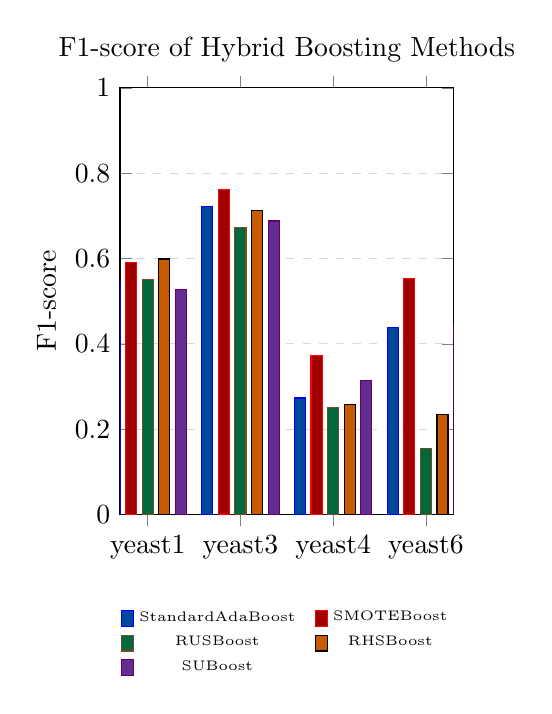
\begin{tikzpicture}
    \begin{axis}[
        ybar,
        height=7cm,
        width=0.48\textwidth,
        bar width=4pt,
        ylabel={F1-score},
        symbolic x coords={yeast1,yeast3,yeast4,yeast6},
        xtick=data,
        ymin=0, ymax=1.0,
        legend style={at={(0.5,-0.2)}, anchor=north, legend columns=2, font=\tiny, draw=none, /tikz/every even column/.append style={column sep=5pt}},
        legend image code/.code={\draw[#1] (0cm,-0.1cm) rectangle (0.15cm,0.1cm);},
        ymajorgrids=true,
        grid style={dashed,gray!30},
        title={F1-score of Hybrid Boosting Methods},
      ]
      \addplot+ [fill=RoyalBlue] coordinates {(yeast1,0.547) (yeast3,0.723) (yeast4,0.273) (yeast6,0.439)};
      \addplot+ [fill=ScholarRed] coordinates {(yeast1,0.590) (yeast3,0.761) (yeast4,0.373) (yeast6,0.554)};
      \addplot+ [fill=ScholarGreen] coordinates {(yeast1,0.550) (yeast3,0.673) (yeast4,0.250) (yeast6,0.155)};
      \addplot+ [fill=ScholarOrange] coordinates {(yeast1,0.599) (yeast3,0.712) (yeast4,0.258) (yeast6,0.234)};
      \addplot+ [fill=ScholarPurple] coordinates {(yeast1,0.528) (yeast3,0.688) (yeast4,0.315) (yeast6,0.446)};
      \legend{StandardAdaBoost, SMOTEBoost, RUSBoost, RHSBoost, SUBoost}
    \end{axis}
  \end{tikzpicture}
  \caption{[Hybrid Method] Performance comparison of various hybrid boosting methods (based on exp\_1.csv).}
  \label{fig:hybrid_boosting}
\end{figure}

\subsubsection{Impact of SMOTE Variants in Hybrid Frameworks}
Figure~\ref{fig:smote_variants} shows the comparative performance of SMOTE-based hybrid strategies. SMOTEBoost demonstrates superior F1-scores compared to the pure data-level SMOTE and the cost-sensitive variant SMOTECSL, particularly as the imbalance ratio increases in Yeast-4 and Yeast-6.

\begin{figure}[h]
  \centering
  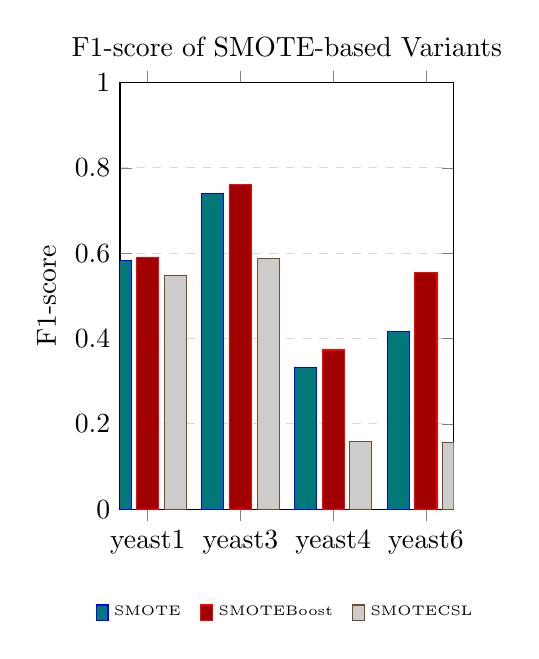
\begin{tikzpicture}
    \begin{axis}[
        ybar,
        height=7cm,
        width=0.48\textwidth,
        bar width=8pt,
        ylabel={F1-score},
        symbolic x coords={yeast1,yeast3,yeast4,yeast6},
        xtick=data,
        ymin=0, ymax=1.0,
        legend style={at={(0.5,-0.2)}, anchor=north, legend columns=-1, font=\tiny, draw=none, /tikz/every even column/.append style={column sep=5pt}},
        legend image code/.code={\draw[#1] (0cm,-0.1cm) rectangle (0.15cm,0.1cm);},
        ymajorgrids=true,
        grid style={dashed,gray!30},
        title={F1-score of SMOTE-based Variants},
      ]
      \addplot+ [fill=ScholarTeal] coordinates {(yeast1,0.583) (yeast3,0.739) (yeast4,0.331) (yeast6,0.416)};
      \addplot+ [fill=ScholarRed] coordinates {(yeast1,0.590) (yeast3,0.761) (yeast4,0.373) (yeast6,0.554)};
      \addplot+ [fill=gray!40] coordinates {(yeast1,0.547) (yeast3,0.588) (yeast4,0.159) (yeast6,0.157)};
      \legend{SMOTE, SMOTEBoost, SMOTECSL}
    \end{axis}
  \end{tikzpicture}
  \caption{[Hybrid Method] Impact of SMOTE variants on model performance (based on exp\_2.csv).}
  \label{fig:smote_variants}
\end{figure}

\subsubsection{ROC Curve Analysis for Hybrid Frameworks}
Figure~\ref{fig:roc_curves} presents the ROC curves of various hybrid boosting methods across the four Yeast datasets. The area under the curve (AUC) provides a summary metric for classification performance.

\begin{figure*}[h]
  \centering
\pgfplotsset{
  roc style/.style={
    xmin=0, xmax=1, ymin=0, ymax=1.02,
    xlabel={False Positive Rate},
    ylabel={True Positive Rate},
    width=7.5cm, height=6.5cm,
    grid=major,
    grid style={dotted, gray!40},
    legend pos=south east,
    legend style={font=\tiny, row sep=-2pt},
    tick label style={font=\footnotesize},
    label style={font=\footnotesize},
    title style={font=\bfseries\small},
  }
}

\begin{tikzpicture}

% ── yeast1 ──
\begin{axis}[
  roc style,
  title={yeast1},
  at={(0cm, 0cm)},
  anchor=north west,
]
\addplot[black, dashed, thick, forget plot] coordinates {(0,0)(1,1)};
\addplot[blue, thick] coordinates {(0.0000,0.0000) (0.0038,0.0280) (0.0066,0.0513) (0.0104,0.0746) (0.0142,0.1049) (0.0171,0.1166) (0.0227,0.1538) (0.0265,0.1772) (0.0303,0.1958) (0.0341,0.2284) (0.0417,0.2448) (0.0445,0.2611) (0.0493,0.2751) (0.0521,0.2890) (0.0578,0.3007) (0.0673,0.3310) (0.0711,0.3403) (0.0787,0.3520) (0.0815,0.3683) (0.0882,0.3776) (0.0929,0.3846) (0.0967,0.4103) (0.1033,0.4242) (0.1090,0.4336) (0.1156,0.4522) (0.1242,0.4755) (0.1289,0.4918) (0.1355,0.5128) (0.1517,0.5198) (0.1564,0.5291) (0.1611,0.5455) (0.1678,0.5571) (0.1773,0.5711) (0.1848,0.5828) (0.1934,0.5897) (0.2038,0.5991) (0.2104,0.6177) (0.2275,0.6247) (0.2455,0.6317) (0.2483,0.6434) (0.2569,0.6550) (0.2635,0.6690) (0.2673,0.6853) (0.2730,0.6970) (0.2900,0.7086) (0.3005,0.7203) (0.3062,0.7273) (0.3128,0.7436) (0.3194,0.7552) (0.3270,0.7622) (0.3365,0.7739) (0.3630,0.7855) (0.3754,0.7925) (0.3820,0.7995) (0.3886,0.8065) (0.4028,0.8135) (0.4142,0.8228) (0.4199,0.8298) (0.4275,0.8415) (0.4588,0.8508) (0.4720,0.8578) (0.4872,0.8648) (0.5100,0.8718) (0.5194,0.8788) (0.5374,0.8858) (0.5744,0.8951) (0.5943,0.9044) (0.6171,0.9114) (0.6370,0.9184) (0.6531,0.9277) (0.6701,0.9371) (0.6768,0.9441) (0.6825,0.9534) (0.7175,0.9604) (0.7555,0.9674) (0.7877,0.9720) (0.8123,0.9790) (0.8701,0.9860) (0.8815,0.9930) (1.0000,1.0000)};
\addlegendentry{AdaBoost\string(depth=5\string) (0.781)}
\addplot[orange!90!black, thick] coordinates {(0.0000,0.0000) (0.0152,0.0956) (0.0161,0.1002) (0.0171,0.1049) (0.0209,0.1096) (0.0246,0.1119) (0.0275,0.1212) (0.0294,0.1329) (0.0332,0.1515) (0.0360,0.1678) (0.0417,0.1841) (0.0464,0.2028) (0.0588,0.2448) (0.0616,0.2587) (0.0626,0.2611) (0.0692,0.2704) (0.0919,0.3520) (0.0938,0.3566) (0.0976,0.3823) (0.1033,0.3893) (0.1071,0.3916) (0.1156,0.4172) (0.1251,0.4406) (0.1280,0.4429) (0.1403,0.4825) (0.1517,0.5198) (0.1630,0.5478) (0.1659,0.5478) (0.1716,0.5618) (0.1801,0.5688) (0.1981,0.6084) (0.1991,0.6200) (0.2028,0.6270) (0.2047,0.6294) (0.2171,0.6457) (0.2218,0.6527) (0.2379,0.6620) (0.2389,0.6643) (0.2464,0.6783) (0.2493,0.6876) (0.2607,0.7040) (0.2682,0.7110) (0.2720,0.7110) (0.2749,0.7179) (0.3043,0.7413) (0.3081,0.7436) (0.3204,0.7459) (0.3299,0.7483) (0.3431,0.7552) (0.3488,0.7552) (0.3630,0.7599) (0.3668,0.7599) (0.4019,0.7879) (0.4171,0.7925) (0.4209,0.8019) (0.4218,0.8042) (0.4303,0.8042) (0.4493,0.8322) (0.4540,0.8368) (0.4645,0.8392) (0.4787,0.8508) (0.4900,0.8531) (0.4948,0.8555) (0.4995,0.8578) (0.5118,0.8578) (0.5204,0.8625) (0.5469,0.8718) (0.5706,0.8858) (0.5782,0.8904) (0.6066,0.8998) (0.6597,0.9301) (0.6863,0.9441) (0.7024,0.9441) (0.7118,0.9464) (0.7336,0.9487) (0.7374,0.9487) (0.7422,0.9557) (0.7649,0.9720) (0.7668,0.9744) (1.0000,1.0000)};
\addlegendentry{SMOTEBoost (0.772)}
\addplot[green!60!black, thick] coordinates {(0.0000,0.0000) (0.0645,0.2657) (0.0645,0.2681) (0.0664,0.2751) (0.0692,0.2774) (0.0720,0.2914) (0.0730,0.2984) (0.0863,0.3170) (0.0919,0.3193) (0.0929,0.3240) (0.0948,0.3310) (0.0986,0.3380) (0.1071,0.3566) (0.1071,0.3636) (0.1100,0.3660) (0.1128,0.3660) (0.1166,0.3869) (0.1213,0.4033) (0.1251,0.4033) (0.1327,0.4196) (0.1327,0.4219) (0.1469,0.4732) (0.1517,0.4848) (0.1545,0.4988) (0.1573,0.5012) (0.1640,0.5105) (0.1668,0.5105) (0.1687,0.5105) (0.1706,0.5152) (0.1716,0.5198) (0.1754,0.5198) (0.1763,0.5221) (0.1886,0.5524) (0.1962,0.5641) (0.2047,0.5734) (0.2123,0.5804) (0.2256,0.5944) (0.2389,0.6084) (0.2408,0.6084) (0.2427,0.6131) (0.2474,0.6270) (0.2645,0.6317) (0.2701,0.6317) (0.3289,0.7063) (0.3299,0.7063) (0.3327,0.7086) (0.3460,0.7133) (0.3479,0.7133) (0.3498,0.7156) (0.3545,0.7179) (0.4057,0.7925) (0.4066,0.7925) (0.4256,0.8019) (0.4360,0.8135) (0.4370,0.8159) (0.4559,0.8298) (0.4711,0.8368) (0.4777,0.8462) (0.4796,0.8462) (0.4900,0.8462) (0.4948,0.8485) (0.5005,0.8508) (0.5175,0.8601) (0.5289,0.8625) (0.5336,0.8625) (0.5336,0.8671) (0.5839,0.8858) (0.5877,0.8881) (0.6019,0.9021) (0.6057,0.9021) (0.6180,0.9068) (0.6341,0.9161) (0.6389,0.9161) (0.6806,0.9510) (0.6834,0.9510) (0.6938,0.9510) (0.7232,0.9604) (0.7336,0.9674) (0.7355,0.9674) (1.0000,1.0000)};
\addlegendentry{RUSBoost (0.757)}
\addplot[red, thick] coordinates {(0.0000,0.0000) (0.0085,0.0536) (0.0085,0.0606) (0.0142,0.0769) (0.0152,0.1072) (0.0171,0.1212) (0.0209,0.1422) (0.0294,0.1772) (0.0303,0.2028) (0.0379,0.2191) (0.0408,0.2284) (0.0455,0.2681) (0.0474,0.2727) (0.0682,0.3193) (0.0796,0.3566) (0.0834,0.3636) (0.0844,0.3753) (0.0872,0.3823) (0.0948,0.3939) (0.0967,0.4009) (0.0986,0.4289) (0.1071,0.4685) (0.1147,0.4779) (0.1166,0.4802) (0.1232,0.4942) (0.1299,0.4988) (0.1384,0.5291) (0.1460,0.5478) (0.1536,0.5594) (0.1564,0.5618) (0.1725,0.5991) (0.1754,0.5991) (0.1782,0.6014) (0.1943,0.6434) (0.2000,0.6434) (0.2066,0.6457) (0.2227,0.6643) (0.2275,0.6737) (0.2303,0.6830) (0.2332,0.6853) (0.2360,0.6876) (0.2455,0.6946) (0.2540,0.7040) (0.2550,0.7063) (0.2768,0.7203) (0.2777,0.7249) (0.2787,0.7273) (0.3033,0.7506) (0.3545,0.7995) (0.3583,0.8042) (0.3725,0.8089) (0.3801,0.8205) (0.3867,0.8228) (0.3915,0.8298) (0.4038,0.8392) (0.4104,0.8462) (0.4152,0.8485) (0.4275,0.8485) (0.4531,0.8601) (0.4626,0.8625) (0.4891,0.8765) (0.4910,0.8788) (0.4967,0.8788) (0.5118,0.8811) (0.5147,0.8811) (0.5213,0.8811) (0.5384,0.8858) (0.5431,0.8858) (0.5526,0.8904) (0.5972,0.9138) (0.6464,0.9254) (0.6711,0.9301) (0.6749,0.9324) (0.6938,0.9441) (0.7166,0.9464) (0.7308,0.9510) (0.7393,0.9557) (0.7526,0.9557) (0.7545,0.9627) (1.0000,1.0000)};
\addlegendentry{RHSBoost (0.791)}
\addplot[violet, thick] coordinates {(0.0000,0.0000) (0.0057,0.0233) (0.0133,0.0746) (0.0180,0.0909) (0.0218,0.1049) (0.0246,0.1259) (0.0275,0.1585) (0.0313,0.1772) (0.0360,0.1841) (0.0398,0.1935) (0.0427,0.2261) (0.0483,0.2354) (0.0540,0.2541) (0.0569,0.2774) (0.0645,0.2960) (0.0682,0.3100) (0.0796,0.3170) (0.0815,0.3310) (0.0882,0.3427) (0.0976,0.3590) (0.1033,0.3753) (0.1062,0.3823) (0.1128,0.3893) (0.1185,0.4009) (0.1261,0.4172) (0.1336,0.4336) (0.1403,0.4429) (0.1479,0.4569) (0.1659,0.4685) (0.1735,0.4802) (0.1763,0.4895) (0.1867,0.5105) (0.1924,0.5221) (0.2000,0.5408) (0.2066,0.5571) (0.2142,0.5641) (0.2256,0.5711) (0.2313,0.5851) (0.2427,0.5967) (0.2493,0.6154) (0.2550,0.6224) (0.2711,0.6364) (0.2758,0.6434) (0.2872,0.6573) (0.3024,0.6667) (0.3137,0.6807) (0.3242,0.6876) (0.3327,0.6993) (0.3517,0.7086) (0.3573,0.7179) (0.3763,0.7249) (0.3820,0.7319) (0.3896,0.7622) (0.4009,0.7739) (0.4209,0.7855) (0.4360,0.7972) (0.4502,0.8042) (0.4578,0.8112) (0.4692,0.8205) (0.4853,0.8298) (0.4995,0.8368) (0.5185,0.8438) (0.5346,0.8625) (0.5507,0.8695) (0.5649,0.8788) (0.5725,0.8858) (0.5791,0.8951) (0.5924,0.9044) (0.6351,0.9114) (0.6398,0.9231) (0.6578,0.9301) (0.6739,0.9394) (0.6995,0.9464) (0.7308,0.9510) (0.7469,0.9604) (0.7592,0.9697) (0.8000,0.9720) (0.8521,0.9814) (0.8900,0.9930) (1.0000,1.0000)};
\addlegendentry{SUBoost (0.754)}
\end{axis}

% ── yeast3 ──
\begin{axis}[
  roc style,
  title={yeast3},
  at={(8.5cm, 0cm)},
  anchor=north west,
]
\addplot[black, dashed, thick, forget plot] coordinates {(0,0)(1,1)};
\addplot[blue, thick] coordinates {(0.0000,0.0000) (0.0000,0.0307) (0.0008,0.0429) (0.0015,0.1043) (0.0023,0.1166) (0.0030,0.2086) (0.0038,0.2331) (0.0061,0.2638) (0.0076,0.2822) (0.0083,0.3129) (0.0091,0.3313) (0.0098,0.3374) (0.0106,0.3620) (0.0114,0.3681) (0.0121,0.4233) (0.0129,0.4294) (0.0136,0.4417) (0.0144,0.4479) (0.0151,0.4969) (0.0159,0.5399) (0.0182,0.5460) (0.0189,0.5767) (0.0212,0.5828) (0.0220,0.5890) (0.0227,0.6074) (0.0235,0.6258) (0.0250,0.6626) (0.0257,0.6748) (0.0265,0.6810) (0.0273,0.6994) (0.0280,0.7055) (0.0295,0.7669) (0.0303,0.7914) (0.0333,0.7975) (0.0356,0.8037) (0.0371,0.8098) (0.0401,0.8160) (0.0439,0.8221) (0.0447,0.8282) (0.0454,0.8344) (0.0469,0.8466) (0.0568,0.8528) (0.0583,0.8589) (0.0613,0.8650) (0.0636,0.8712) (0.0696,0.8773) (0.0749,0.8834) (0.0931,0.8896) (0.0969,0.8957) (0.1022,0.9018) (0.1045,0.9080) (0.1105,0.9141) (0.1249,0.9202) (0.1272,0.9264) (0.1355,0.9325) (0.1393,0.9387) (0.1431,0.9448) (0.1499,0.9509) (0.2044,0.9509) (0.2051,0.9571) (0.2831,0.9571) (0.2854,0.9571) (0.2869,0.9632) (0.2952,0.9693) (0.3202,0.9693) (0.3338,0.9755) (0.3702,0.9816) (0.4943,0.9877) (0.5799,0.9939) (0.5973,0.9939) (0.6457,0.9939) (0.6858,0.9939) (0.7638,0.9939) (0.8486,1.0000) (0.8622,1.0000) (0.8819,1.0000) (0.8849,1.0000) (0.9258,1.0000) (0.9796,1.0000) (1.0000,1.0000)};
\addlegendentry{AdaBoost\string(depth=5\string) (0.958)}
\addplot[orange!90!black, thick] coordinates {(0.0000,0.0000) (0.0023,0.0798) (0.0030,0.1166) (0.0038,0.1595) (0.0045,0.1840) (0.0053,0.3681) (0.0053,0.3988) (0.0061,0.4049) (0.0076,0.4294) (0.0083,0.4356) (0.0091,0.4601) (0.0106,0.4601) (0.0114,0.4724) (0.0129,0.5031) (0.0151,0.5276) (0.0167,0.5337) (0.0167,0.5706) (0.0174,0.5951) (0.0182,0.6135) (0.0197,0.6258) (0.0204,0.6319) (0.0235,0.6564) (0.0250,0.6564) (0.0257,0.6748) (0.0273,0.6933) (0.0280,0.7239) (0.0288,0.7362) (0.0288,0.7423) (0.0303,0.7607) (0.0318,0.7730) (0.0326,0.7853) (0.0348,0.7975) (0.0379,0.7975) (0.0394,0.8037) (0.0401,0.8098) (0.0409,0.8160) (0.0447,0.8221) (0.0447,0.8282) (0.0477,0.8344) (0.0530,0.8405) (0.0537,0.8466) (0.0560,0.8528) (0.0568,0.8589) (0.0575,0.8589) (0.0727,0.8712) (0.0734,0.8773) (0.0749,0.8896) (0.0802,0.8957) (0.0802,0.9018) (0.0840,0.9141) (0.0908,0.9202) (0.0931,0.9264) (0.0946,0.9325) (0.1007,0.9325) (0.1400,0.9387) (0.1802,0.9448) (0.1847,0.9509) (0.1862,0.9571) (0.1862,0.9632) (0.2377,0.9632) (0.2816,0.9693) (0.2877,0.9693) (0.3588,0.9755) (0.3603,0.9877) (0.5026,0.9877) (0.5291,0.9877) (0.5882,0.9877) (0.5988,0.9877) (0.6177,0.9877) (0.6192,0.9877) (0.7055,0.9877) (0.7782,0.9939) (0.8213,0.9939) (0.8584,0.9939) (0.8698,0.9939) (0.8812,0.9939) (0.9243,0.9939) (0.9364,1.0000) (0.9917,1.0000) (1.0000,1.0000)};
\addlegendentry{SMOTEBoost (0.959)}
\addplot[green!60!black, thick] coordinates {(0.0000,0.0000) (0.0553,0.7301) (0.0560,0.7301) (0.0560,0.7546) (0.0568,0.7607) (0.0583,0.7607) (0.0598,0.7607) (0.0621,0.7669) (0.0628,0.7669) (0.0651,0.7730) (0.0651,0.7791) (0.0681,0.7853) (0.0689,0.7975) (0.0719,0.8037) (0.0719,0.8160) (0.0742,0.8405) (0.0810,0.8589) (0.0855,0.8896) (0.0878,0.9080) (0.0901,0.9080) (0.0977,0.9080) (0.0984,0.9141) (0.1022,0.9202) (0.1090,0.9202) (0.1173,0.9202) (0.1196,0.9202) (0.1204,0.9264) (0.1219,0.9264) (0.1257,0.9264) (0.1287,0.9264) (0.1385,0.9387) (0.1416,0.9387) (0.1522,0.9448) (0.1605,0.9448) (0.1787,0.9448) (0.1802,0.9448) (0.1840,0.9448) (0.1862,0.9509) (0.1968,0.9509) (0.2036,0.9509) (0.2036,0.9571) (0.2044,0.9571) (0.2082,0.9571) (0.2097,0.9571) (0.2120,0.9571) (0.2180,0.9571) (0.2210,0.9571) (1.0000,1.0000)};
\addlegendentry{RUSBoost (0.934)}
\addplot[red, thick] coordinates {(0.0000,0.0000) (0.0341,0.7546) (0.0356,0.7546) (0.0356,0.7607) (0.0363,0.7669) (0.0386,0.7669) (0.0401,0.7669) (0.0424,0.7853) (0.0469,0.7914) (0.0530,0.8037) (0.0553,0.8160) (0.0560,0.8160) (0.0606,0.8344) (0.0643,0.8344) (0.0643,0.8405) (0.0643,0.8528) (0.0659,0.8528) (0.0681,0.8712) (0.0719,0.8773) (0.0727,0.8773) (0.0765,0.9018) (0.0772,0.9018) (0.0787,0.9018) (0.0818,0.9018) (0.0924,0.9202) (0.0946,0.9264) (0.0977,0.9387) (0.0999,0.9448) (0.1007,0.9448) (0.1083,0.9448) (0.1113,0.9448) (0.1173,0.9448) (0.1325,0.9448) (0.1332,0.9448) (0.1544,0.9571) (0.1552,0.9571) (0.1718,0.9632) (0.1726,0.9632) (0.1756,0.9632) (0.1771,0.9632) (0.1824,0.9632) (0.1832,0.9632) (0.1870,0.9632) (0.1923,0.9693) (0.1953,0.9693) (0.1968,0.9693) (0.1998,0.9755) (0.2029,0.9755) (0.2067,0.9755) (1.0000,1.0000)};
\addlegendentry{RHSBoost (0.955)}
\addplot[violet, thick] coordinates {(0.0000,0.0000) (0.0008,0.0123) (0.0015,0.0184) (0.0023,0.0245) (0.0030,0.0920) (0.0045,0.0982) (0.0053,0.1043) (0.0061,0.2209) (0.0068,0.2331) (0.0083,0.2822) (0.0091,0.3006) (0.0098,0.3436) (0.0106,0.3558) (0.0121,0.3620) (0.0136,0.3804) (0.0144,0.3865) (0.0151,0.4417) (0.0159,0.4908) (0.0174,0.5399) (0.0182,0.5583) (0.0189,0.5706) (0.0204,0.6258) (0.0250,0.6319) (0.0295,0.6810) (0.0326,0.6871) (0.0333,0.6933) (0.0401,0.7055) (0.0469,0.7362) (0.0500,0.7423) (0.0515,0.7485) (0.0530,0.7607) (0.0613,0.7607) (0.0787,0.7607) (0.0795,0.7669) (0.0863,0.7669) (0.0886,0.7730) (0.0916,0.7853) (0.0946,0.7914) (0.0961,0.8098) (0.1007,0.8160) (0.1067,0.8221) (0.1090,0.8282) (0.1113,0.8344) (0.1181,0.8405) (0.1257,0.8650) (0.1287,0.8712) (0.1294,0.8773) (0.1310,0.8834) (0.1347,0.8896) (0.1506,0.8957) (0.1575,0.9080) (0.1665,0.9141) (0.1787,0.9202) (0.1817,0.9325) (0.1855,0.9387) (0.1893,0.9448) (0.2369,0.9571) (0.2400,0.9632) (0.2445,0.9693) (0.2551,0.9693) (0.2801,0.9755) (0.3089,0.9816) (0.3301,0.9877) (0.3520,0.9877) (0.4572,0.9877) (0.4671,0.9877) (0.6563,0.9877) (0.7025,0.9877) (0.7237,0.9877) (0.7615,0.9877) (0.7812,0.9877) (0.7971,0.9877) (0.8002,0.9877) (0.8153,0.9877) (0.8319,0.9877) (0.8577,0.9939) (0.8615,0.9939) (0.8849,0.9939) (0.8872,0.9939) (1.0000,1.0000)};
\addlegendentry{SUBoost (0.943)}
\end{axis}

% ── yeast4 ──
\begin{axis}[
  roc style,
  title={yeast4},
  at={(0cm, -7.5cm)},
  anchor=north west,
]
\addplot[black, dashed, thick, forget plot] coordinates {(0,0)(1,1)};
\addplot[blue, thick] coordinates {(0.0000,0.0000) (0.0000,0.0196) (0.0007,0.0196) (0.0014,0.0588) (0.0014,0.1176) (0.0021,0.1373) (0.0028,0.1373) (0.0070,0.1569) (0.0070,0.1961) (0.0098,0.2157) (0.0105,0.2157) (0.0112,0.2549) (0.0112,0.2745) (0.0119,0.2941) (0.0133,0.2941) (0.0161,0.3137) (0.0161,0.3529) (0.0188,0.3529) (0.0195,0.3725) (0.0195,0.3922) (0.0202,0.4118) (0.0258,0.4118) (0.0279,0.4314) (0.0286,0.4510) (0.0321,0.4706) (0.0321,0.4902) (0.0412,0.5098) (0.0440,0.5098) (0.0495,0.5294) (0.0495,0.5686) (0.0502,0.5882) (0.0537,0.5882) (0.0537,0.6078) (0.0572,0.6275) (0.0579,0.6275) (0.0677,0.6471) (0.0677,0.6667) (0.0712,0.6863) (0.0782,0.6863) (0.0830,0.7059) (0.0844,0.7059) (0.0893,0.7451) (0.0893,0.7647) (0.0970,0.7843) (0.1221,0.7843) (0.1284,0.8039) (0.1284,0.8235) (0.1326,0.8431) (0.1375,0.8431) (0.1375,0.8627) (0.1417,0.8824) (0.1465,0.8824) (0.1493,0.9020) (0.1493,0.9216) (0.1766,0.9216) (0.1933,0.9216) (0.2401,0.9412) (0.2415,0.9412) (0.2736,0.9608) (0.4829,0.9608) (0.4850,0.9608) (0.4850,0.9804) (0.4913,1.0000) (0.5359,1.0000) (0.5373,1.0000) (0.5527,1.0000) (0.6120,1.0000) (0.6288,1.0000) (0.6301,1.0000) (0.6992,1.0000) (0.7027,1.0000) (0.7202,1.0000) (0.7216,1.0000) (0.7983,1.0000) (0.8702,1.0000) (0.9400,1.0000) (0.9414,1.0000) (0.9707,1.0000) (0.9721,1.0000) (1.0000,1.0000)};
\addlegendentry{AdaBoost\string(depth=5\string) (0.928)}
\addplot[orange!90!black, thick] coordinates {(0.0000,0.0000) (0.0007,0.0000) (0.0007,0.0196) (0.0014,0.0196) (0.0021,0.0588) (0.0021,0.0980) (0.0028,0.0980) (0.0028,0.1176) (0.0035,0.2157) (0.0056,0.2157) (0.0056,0.2549) (0.0063,0.2941) (0.0077,0.2941) (0.0077,0.3137) (0.0119,0.3137) (0.0140,0.3333) (0.0140,0.3529) (0.0195,0.3529) (0.0265,0.3725) (0.0265,0.3922) (0.0272,0.3922) (0.0272,0.4118) (0.0328,0.4314) (0.0433,0.4314) (0.0433,0.4510) (0.0475,0.4510) (0.0482,0.4706) (0.0482,0.5294) (0.0488,0.5294) (0.0565,0.5490) (0.0565,0.5686) (0.0670,0.5686) (0.0670,0.5882) (0.0719,0.6078) (0.0789,0.6078) (0.0789,0.6471) (0.0816,0.6667) (0.0823,0.6667) (0.0823,0.6863) (0.0858,0.6863) (0.0872,0.7059) (0.0872,0.7255) (0.1026,0.7255) (0.1026,0.7451) (0.1124,0.7647) (0.1137,0.7647) (0.1137,0.7843) (0.1291,0.8235) (0.1340,0.8235) (0.1340,0.8431) (0.1445,0.8431) (0.1661,0.8627) (0.1661,0.8824) (0.1842,0.8824) (0.2275,0.9020) (0.2275,0.9216) (0.3733,0.9216) (0.3733,0.9412) (0.4159,0.9608) (0.4368,0.9608) (0.4368,0.9804) (0.5827,0.9804) (0.6036,0.9804) (0.6050,0.9804) (0.6567,0.9804) (0.6588,0.9804) (0.6602,0.9804) (0.7111,0.9804) (0.7125,0.9804) (0.7893,1.0000) (0.7900,1.0000) (0.7913,1.0000) (0.8618,1.0000) (0.8632,1.0000) (0.8646,1.0000) (0.9630,1.0000) (0.9798,1.0000) (0.9812,1.0000) (0.9819,1.0000) (1.0000,1.0000)};
\addlegendentry{SMOTEBoost (0.909)}
\addplot[green!60!black, thick] coordinates {(0.0000,0.0000) (0.1082,0.7255) (0.1096,0.7255) (0.1110,0.7451) (0.1117,0.7647) (0.1144,0.7647) (0.1186,0.7647) (0.1242,0.7647) (0.1242,0.7843) (0.1291,0.8039) (0.1298,0.8039) (0.1354,0.8235) (0.1452,0.8235) (0.1465,0.8431) (0.1528,0.8431) (0.1598,0.8431) (0.1626,0.8431) (0.1752,0.8431) (0.1779,0.8431) (0.1849,0.8431) (0.1982,0.8431) (0.2219,0.8824) (0.2233,0.8824) (0.2240,0.9020) (0.2261,0.9020) (0.2324,0.9216) (0.2373,0.9216) (0.2456,0.9216) (0.2589,0.9216) (0.2596,0.9216) (0.2610,0.9412) (0.2617,0.9412) (1.0000,1.0000)};
\addlegendentry{RUSBoost (0.887)}
\addplot[red, thick] coordinates {(0.0000,0.0000) (0.1012,0.7255) (0.1019,0.7255) (0.1047,0.7255) (0.1082,0.7255) (0.1144,0.7451) (0.1172,0.7451) (0.1186,0.7451) (0.1249,0.7647) (0.1256,0.7647) (0.1270,0.7647) (0.1312,0.7647) (0.1333,0.7647) (0.1361,0.7647) (0.1375,0.7843) (0.1396,0.7843) (0.1528,0.7843) (0.1542,0.7843) (0.1549,0.7843) (0.1591,0.8039) (0.1598,0.8039) (0.1619,0.8039) (0.1633,0.8039) (0.1640,0.8235) (0.1654,0.8235) (0.1675,0.8431) (0.1703,0.8431) (0.1877,0.8824) (0.1975,0.8824) (0.1982,0.8824) (0.2100,0.8824) (0.2100,0.9020) (0.2128,0.9020) (0.2240,0.9216) (0.2296,0.9216) (0.2303,0.9216) (1.0000,1.0000)};
\addlegendentry{RHSBoost (0.883)}
\addplot[violet, thick] coordinates {(0.0000,0.0000) (0.0007,0.0196) (0.0014,0.0588) (0.0028,0.0784) (0.0112,0.1569) (0.0140,0.2157) (0.0167,0.2549) (0.0174,0.2941) (0.0216,0.3137) (0.0237,0.3333) (0.0258,0.3725) (0.0314,0.3922) (0.0342,0.4314) (0.0377,0.4510) (0.0391,0.4902) (0.0405,0.5098) (0.0454,0.5294) (0.0502,0.5490) (0.0614,0.5686) (0.0635,0.5686) (0.0782,0.5882) (0.0858,0.6275) (0.0907,0.6275) (0.1005,0.6275) (0.1151,0.6471) (0.1291,0.6471) (0.1347,0.6471) (0.1368,0.6471) (0.1424,0.6471) (0.1465,0.6471) (0.1549,0.6471) (0.1633,0.6471) (0.1668,0.6471) (0.1710,0.6471) (0.1766,0.6471) (0.1898,0.6667) (0.2100,0.6667) (0.2142,0.6863) (0.2212,0.6863) (0.2282,0.6863) (0.2352,0.6863) (0.2373,0.7059) (0.2533,0.7255) (0.2610,0.7255) (0.2666,0.7255) (0.2694,0.7255) (0.2826,0.7255) (0.2959,0.7255) (0.3001,0.7255) (0.3070,0.7255) (0.3098,0.7255) (0.3161,0.7255) (0.3266,0.7255) (0.3308,0.7255) (0.3343,0.7255) (0.3503,0.7451) (0.3629,0.7647) (0.4040,0.7843) (0.4313,0.8039) (0.4382,0.8431) (0.4389,0.8627) (0.4410,0.8824) (0.5213,0.9020) (0.5227,0.9216) (0.6176,0.9412) (0.7041,0.9412) (0.7327,0.9412) (0.7565,0.9412) (0.7844,0.9412) (0.7976,0.9412) (0.8325,0.9412) (0.8339,0.9608) (0.8500,0.9804) (0.9114,0.9804) (0.9546,1.0000) (0.9574,1.0000) (0.9658,1.0000) (0.9833,1.0000) (0.9867,1.0000) (1.0000,1.0000)};
\addlegendentry{SUBoost (0.820)}
\end{axis}

% ── yeast6 ──
\begin{axis}[
  roc style,
  title={yeast6},
  at={(8.5cm, -7.5cm)},
  anchor=north west,
]
\addplot[black, dashed, thick, forget plot] coordinates {(0,0)(1,1)};
\addplot[blue, thick] coordinates {(0.0000,0.0000) (0.0000,0.0286) (0.0014,0.1143) (0.0021,0.1429) (0.0021,0.2571) (0.0028,0.2857) (0.0035,0.3143) (0.0041,0.3143) (0.0062,0.3429) (0.0083,0.3714) (0.0097,0.4000) (0.0097,0.4286) (0.0104,0.4857) (0.0110,0.5429) (0.0124,0.5429) (0.0138,0.5714) (0.0297,0.6000) (0.0524,0.6286) (0.0524,0.6571) (0.0594,0.6857) (0.0635,0.7143) (0.0987,0.7143) (0.1718,0.7429) (0.1946,0.7714) (0.2112,0.7714) (0.2126,0.7714) (0.2181,0.8000) (0.2346,0.8286) (0.2429,0.8286) (0.2740,0.8571) (0.2947,0.8571) (0.2947,0.8857) (0.3202,0.8857) (0.3464,0.8857) (0.3789,0.8857) (0.3844,0.8857) (0.4493,0.9143) (0.4610,0.9429) (0.4624,0.9429) (0.4748,0.9429) (0.5204,0.9429) (0.5266,0.9429) (0.5293,0.9429) (0.5424,0.9429) (0.5887,0.9429) (0.5901,0.9429) (0.5977,0.9429) (0.6197,0.9429) (0.6577,0.9429) (0.6625,0.9429) (0.6687,0.9429) (0.6756,0.9429) (0.6770,0.9429) (0.6977,0.9429) (0.7012,0.9429) (0.7129,0.9429) (0.7191,0.9714) (0.7329,0.9714) (0.7474,0.9714) (0.7495,0.9714) (0.7591,0.9714) (0.7847,0.9714) (0.8406,0.9714) (0.8447,0.9714) (0.8758,0.9714) (0.8820,0.9714) (0.8834,0.9714) (0.8882,0.9714) (0.9055,0.9714) (0.9275,0.9714) (0.9455,0.9714) (0.9510,0.9714) (0.9614,0.9714) (0.9614,1.0000) (0.9683,1.0000) (0.9745,1.0000) (0.9765,1.0000) (0.9807,1.0000) (0.9855,1.0000) (1.0000,1.0000)};
\addlegendentry{AdaBoost\string(depth=5\string) (0.883)}
\addplot[orange!90!black, thick] coordinates {(0.0000,0.0000) (0.0000,0.0286) (0.0000,0.1143) (0.0007,0.1143) (0.0014,0.1429) (0.0014,0.2286) (0.0021,0.2286) (0.0028,0.2571) (0.0028,0.3429) (0.0035,0.3429) (0.0041,0.4000) (0.0041,0.4571) (0.0062,0.4571) (0.0062,0.4857) (0.0083,0.5429) (0.0104,0.5429) (0.0104,0.5714) (0.0110,0.6000) (0.0131,0.6000) (0.0131,0.6286) (0.0166,0.6571) (0.0173,0.6571) (0.0173,0.6857) (0.0483,0.6857) (0.0663,0.7143) (0.0663,0.7429) (0.0718,0.7429) (0.0807,0.7714) (0.0814,0.8000) (0.0904,0.8000) (0.1070,0.8000) (0.1084,0.8000) (0.1111,0.8000) (0.1159,0.8000) (0.1173,0.8000) (0.2174,0.8000) (0.2174,0.8286) (0.2250,0.8571) (0.3354,0.8571) (0.3354,0.8857) (0.3589,0.9143) (0.4596,0.9143) (0.4610,0.9143) (0.5169,0.9143) (0.5562,0.9143) (0.5576,0.9143) (0.5638,0.9143) (0.5687,0.9143) (0.5687,0.9429) (0.5735,0.9429) (0.6142,0.9429) (0.6156,0.9429) (0.6253,0.9429) (0.6329,0.9429) (0.6329,0.9714) (0.6743,0.9714) (0.6846,0.9714) (0.6860,0.9714) (0.7191,0.9714) (0.7205,0.9714) (0.7474,1.0000) (0.7488,1.0000) (0.7502,1.0000) (0.7854,1.0000) (0.8068,1.0000) (0.8081,1.0000) (0.8233,1.0000) (0.8737,1.0000) (0.8751,1.0000) (0.8896,1.0000) (0.9199,1.0000) (0.9213,1.0000) (0.9600,1.0000) (0.9634,1.0000) (0.9648,1.0000) (0.9710,1.0000) (0.9869,1.0000) (0.9883,1.0000) (0.9959,1.0000) (1.0000,1.0000)};
\addlegendentry{SMOTEBoost (0.901)}
\addplot[green!60!black, thick] coordinates {(0.0000,0.0000) (0.1663,0.8286) (0.1670,0.8286) (0.1691,0.8286) (0.1753,0.8286) (0.1760,0.8286) (0.1774,0.8286) (0.1822,0.8286) (0.1836,0.8286) (0.1925,0.8286) (0.2367,0.8286) (0.2381,0.8286) (0.2478,0.8286) (0.2491,0.8286) (0.2622,0.8286) (0.2692,0.8286) (0.2767,0.8286) (1.0000,1.0000)};
\addlegendentry{RUSBoost (0.822)}
\addplot[red, thick] coordinates {(0.0000,0.0000) (0.1201,0.8571) (0.1249,0.8571) (0.1256,0.8571) (0.1297,0.8571) (0.1339,0.8571) (0.1484,0.8571) (0.1518,0.8571) (0.1587,0.8571) (0.1643,0.8571) (0.1663,0.8571) (1.0000,1.0000)};
\addlegendentry{RHSBoost (0.865)}
\addplot[violet, thick] coordinates {(0.0000,0.0000) (0.0007,0.0857) (0.0041,0.1714) (0.0048,0.2857) (0.0076,0.4286) (0.0131,0.4286) (0.0207,0.4571) (0.0269,0.4857) (0.0290,0.5429) (0.0366,0.5429) (0.0386,0.5714) (0.0442,0.6000) (0.0511,0.6000) (0.0566,0.6000) (0.0752,0.6000) (0.0780,0.6286) (0.0856,0.6286) (0.0883,0.6571) (0.0966,0.6571) (0.1077,0.6571) (0.1215,0.6571) (0.1387,0.6571) (0.1422,0.6857) (0.1484,0.6857) (0.1684,0.6857) (0.2050,0.6857) (0.2208,0.7429) (0.2395,0.7714) (0.2664,0.8000) (0.3237,0.8286) (0.3368,0.8571) (0.3596,0.8571) (0.3747,0.8571) (0.3782,0.8571) (0.3823,0.8571) (0.4141,0.8571) (0.4203,0.8571) (0.4362,0.8571) (0.4541,0.8571) (0.4638,0.8571) (0.4769,0.8571) (0.4941,0.8571) (0.5031,0.8571) (0.5266,0.8571) (0.5314,0.8571) (0.5411,0.8571) (0.5542,0.8571) (0.5700,0.8571) (0.5756,0.8571) (0.6108,0.8571) (0.6149,0.8571) (0.6190,0.8571) (0.6294,0.8857) (0.6377,0.8857) (0.6439,0.9143) (0.6501,0.9429) (0.6563,0.9429) (0.6639,0.9429) (0.6950,0.9429) (0.7095,0.9429) (0.7164,0.9429) (0.7219,0.9429) (0.7302,0.9429) (0.7329,0.9429) (0.7495,0.9429) (0.7536,0.9714) (0.7667,0.9714) (0.7716,0.9714) (0.7785,0.9714) (0.7950,0.9714) (0.8585,0.9714) (0.8620,0.9714) (0.8703,0.9714) (0.8772,0.9714) (0.9061,1.0000) (0.9158,1.0000) (0.9814,1.0000) (0.9862,1.0000) (0.9896,1.0000) (1.0000,1.0000)};
\addlegendentry{SUBoost (0.840)}
\end{axis}

\end{tikzpicture}
  \caption{[Hybrid Method] ROC Curve comparison across yeast1, yeast3, yeast4, and yeast6.}
  \label{fig:roc_curves}
\end{figure*}

\subsection{Summary Statement}
The experimental results demonstrate that while data-level methods provide a foundational improvement, algorithm-level and hybrid approaches offer superior stability and performance across extreme imbalance ratios.

\bibliographystyle{ACM-Reference-Format}
\bibliography{sample-base}

\end{document}
